\documentclass[11pt,a4paper]{article}
\usepackage[margin=2cm]{geometry}
\usepackage{indentfirst}
\usepackage[utf8]{inputenc}
\usepackage[T1]{fontenc}
\usepackage{longtable}
\usepackage{booktabs}
\usepackage{array}
\usepackage{graphicx}
\usepackage{titling}
\usepackage{float}
\usepackage{hyperref}
\usepackage{tikz}
\usepackage{amsmath}
\usetikzlibrary{shapes, arrows, positioning}
\usepackage[justification=centering]{caption}
\usetikzlibrary{shapes.geometric, arrows.meta, positioning}
\geometry{left=1.5cm, right=1.5cm, top=2cm, bottom=2cm}
 
\renewcommand{\maketitle}{%
  \begin{titlepage}
    \centering
    
    \vspace*{0.6cm}
 
    {\LARGE \textbf{EVALUASI TENGAH SEMESTER} \\[0.4cm]
     \LARGE \textbf{MATA KULIAH PEMROGRAMAN KONTROLLER}}
 
    \vspace{0.6cm}
 
    {\large \textbf{Dosen Pengampu: Ahmad Radhy, S.Si., M.Si}}
 
    \vspace{1.2cm}
 
    
\includegraphics[width=10cm]{its_logo.png}
 
    \vspace{2cm}
 
    {\normalsize Disusun oleh (Kelompok 9):} \\[0.4cm]
    {\large \textbf{Mahendra Dwi Fahreza} \normalsize (NRP: 2042241023)} \\[0.25cm]
    {\large \textbf{Athaya Zhafari Saputra} \normalsize (NRP: 2042241019)} \\[0.25cm]
    {\normalsize Kelas: \textbf{4B}}
 
    \vfill
 
    {\normalsize
      \textbf{PRODI D4 TEKNOLOGI REKAYASA INSTRUMENTASI} \\[0.2cm]
      \textbf{DEPARTEMEN TEKNIK INSTRUMENTASI} \\[0.2cm]
      \textbf{FAKULTAS VOKASI} \\[0.2cm]
      \textbf{INSTITUT TEKNOLOGI SEPULUH NOPEMBER} \\[0.2cm]
      \textbf{2026}%
    }
 
  \end{titlepage}%
}
 
\title{}
\author{}
\date{}
 
\begin{document}
\maketitle

\section*{A. Studi Literatur}

Bagian ini menyajikan analisis komprehensif terhadap 15 artikel jurnal ilmiah internasional bereputasi yang bersumber dari pangkalan data Scopus dan Web of Science (WoS) dalam rentang publikasi tahun 2021 hingga 2026. Kajian pustaka ini difokuskan secara terarah pada penelusuran topik teknologi dan perkembangan kontroler, dasar serta arsitektur mikrokontroler, pengelolaan periferal sistem benam, \textit{embedded programming}, hingga implementasi \textit{safety-critical system} pada sistem tertanam. Ringkasan dari keseluruhan tata metodologi, hasil utama, beserta arah \textit{future work} yang disarankan oleh masing-masing peneliti disajikan secara terstruktur pada Tabel 1 di bawah ini.

\begin{small}
\begin{longtable}{|c|>{\raggedright\arraybackslash}p{3.2cm}|>{\raggedright\arraybackslash}p{4cm}|>{\raggedright\arraybackslash}p{4cm}|>{\raggedright\arraybackslash}p{4cm}|}
\caption{Ringkasan 15 Jurnal Acuan (2021--2026)} \label{tab:literatur} \\
\hline
\textbf{No} & \textbf{Judul \& Penulis (Tahun)} & \textbf{Metode} & \textbf{Hasil Utama} & \textbf{Future Work} \\
\hline
\endfirsthead
\caption[]{Ringkasan 15 Jurnal Acuan (2021--2026)} \\
\hline
\textbf{No} & \textbf{Judul \& Penulis (Tahun)} & \textbf{Metode} & \textbf{Hasil Utama} & \textbf{Future Work} \\
\hline
\endhead
\hline
\endfoot


1 & A versatile logic-gated fluorescence turn-on nitrogen-doped carbon dots: STM32 microcontroller intelligent platform for assay of L-Histidine and $\text{Al}^{3+}$ \newline \newline \textit{Yong-qing Liu, Bo-wen An, Tao Zhu, Rui-yong Jiang, Ye Wang, Chan Huang, Su-qian Cai, Bi-xiao Zhang, Yan-li Leng, Jing-zhen Pan, Le Liang, Xiao-hua Cai (2026)} & Penelitian ini mengembangkan Nitrogen-doped Carbon Dots (N-CDs) melalui proses hidrotermal sederhana untuk mendeteksi L-His dan $\text{Al}^{3+}$. Metode ini diintegrasikan ke dalam platform sensor cerdas portabel yang digerakkan oleh mikrokontroler STM32 dengan algoritma ratiometrik khusus. Mekanisme penginderaan divalidasi dengan pengukuran TCSPC dan kalkulasi teoritis (DFT dan IGMH). & Hasil penelitian ini N-CDs mencapai batas deteksi (LODs) yang sangat rendah, yaitu $0.950\ \mu\text{M}$ untuk L-His dan $4.393\ \mu\text{M}$ untuk $\text{Al}^{3+}$. Mikrokontroler STM32 sukses melakukan komputasi algoritma untuk analisis kuantitatif on-site, yang secara efektif menjembatani celah antara eksperimen material nano di laboratorium dengan aplikasi praktis di lapangan. & Penulis untuk kedepan berfokus pada upaya meminiaturisasi lebih lanjut desain sirkuit untuk mengintegrasikan modul sensor ke dalam perangkat yang dapat dikenakan (wearable devices) atau sistem IoT, dengan tujuan utama untuk mencapai pemantauan kesehatan yang komprehensif dan penilaian kondisi lingkungan yang berkelanjutan secara real-time di masa mendatang. \\

\hline
2 & Adaptive Microprocessor-Based Interval Type-2 Fuzzy Logic Controller Design for DC Micro-Motor Control Considering Hardware Limitations \newline \newline \textit{Nikolaos V. Chatzipapas, Yannis L. Karnavas (2025)} & Studi ini mensintesis arsitektur pengontrol Interval Type-2 Fuzzy Logic (IT2FLC) yang didesain secara spesifik pada mikrokontroler STM32 berbiaya rendah guna mengemudikan aktuator motor mikro DC coreless. Proses optimasi mengandalkan Particle Swarm Optimization (PSO) real-time demi mematuhi ketatnya batasan memori RAM serta ruang komputasi internal perangkat keras yang terbatas. & Algoritma ini sukses dieksekusi mandiri dengan kestabilan tinggi. Implementasi Type-2 Fuzzy Logic terbukti jauh lebih tangguh meredam overshoot serta fluktuasi torsi motor daripada metode PI/PID/PIDF klasik. Pendekatan hardware-in-the-loop berhasil mematahkan risiko kelebihan muatan komputasi ataupun memory overflow yang kerap melumpuhkan mikrokontroler pada sistem siklus tertutup. & Pengembangan ke depan ditargetkan untuk menyempurnakan kendala perangkat keras secara praktis dan ekstensif. Fokus riset selanjutnya bakal diarahkan untuk mengatasi masalah kompromi antara resolusi kontrol dan frekuensi PWM, sekaligus mencari titik keseimbangan absolut terhadap batas minimal tingkat akurasi pembacaan ukuran sensor enkoder poros motor mikro. \\
\hline

3 & An embedded accelerated decentralized optimization algorithm with application to energy communities \newline \newline \textit{Giulio Ferro, Sergio Grammatico, Luca Parodi, Reza Rahimi Baghbadorani, Michela Robba (2026)} & Penelitian ini memfokuskan pada inovasi embedded programming bersistem desentralisasi untuk mengelola Renewable Energy Communities (REC). Optimasi dijabarkan dalam rumusan Quadratic Programming (QP) dan dieksekusi melalui kode Alternating Direction Method of Multipliers (ADMM) yang dimodifikasi dengan akselerasi matematis Nesterov untuk menjamin kecepatan konvergensi iterasi pemrograman perangkat keras. & Eksperimen komputasi membuktikan mikrokontroler ODROID sukses menjalankan optimasi matriks desentralisasi secara stabil untuk skenario jaringan REC beranggotakan sepuluh partisipan. Eksekusi kode berbasis ADMM mampu menghasilkan penjadwalan presisi tinggi dalam batas waktu operasional real-time tanpa memerlukan pusat pertukaran variabel data secara eksternal, sehingga menjamin kerahasiaan penuh privasi partisipan. & Penulis merekomendasikan modifikasi program agar struktur embedded dapat menangani utilitas jaringan publik secara langsung sekaligus mengintegrasikan kebijakan program respons permintaan. Selanjutnya untuk memitigasi fluktuasi cuaca, penulis akan menyematkan model pemrograman prediksi peramalan cuaca ke dalam sistem, serta mentransisikan algoritma deterministik menjadi metode optimasi stokastik berbasis skenario. \\
\hline

4 & Microcontroller-based numerical control DC stabilized power supply: design, implementation, and performance evaluation \newline \newline \textit{Habib Khan, Liu Yangbin, Hamedalneel B.A. Hamid, Anwar Shahid, Tianjun Ma, Jamal N.A. Hassan, Chingmai Ko, Naeem Ahmed, Wang Yong (2026)} & Penelitian ini mendesain power supply DC terkontrol digital menggunakan mikrokontroler STC89C52RC secara closed-loop. Pendekatannya memadukan perangkat keras dan lunak dengan memanfaatkan dua chip DAC 10-bit untuk menghasilkan referensi tegangan presisi, serta chip ADC 8-bit guna membaca feedback tegangan dan arus secara real-time untuk validasi kalibrasi. & Prototipe yang dikembangkan berhasil memvalidasi penyesuaian tegangan output secara kontinu dari nol sampai dua belas Volt dengan deviasi akurasi tinggi. Mekanisme proteksi perangkat lunak terbukti merespons cepat secara otomatis dengan memutus daya saat ambang batas terlampaui. Secara keseluruhan, sistem beroperasi sangat stabil, responsif, dan sukses menekan biaya produksi. & Penulis mengusulkan saran peningkatan kemampuan anti-interferensi dan mengintegrasikan perangkat ADC yang lebih mutakhir guna mencapai akuisisi data berpresisi tinggi. Selanjutnya penerapan strategi perlindungan hibrida untuk meminimalkan jeda respons yang saat ini masih menjadi kelemahan, serta melengkapi sistem dengan algoritma kontrol adaptif seperti kontrol cerdas PID. \\
\hline

5 & Design a low-cost solar PV data logger and assess the application and accuracy with off-grid monocrystalline panels \newline \newline \textit{MD Shouquat Hossain, Mohamed Bashir Ali Bashir, Khadiza Akter (2026)} & Penelitian ini membangun data logger kelistrikan dan termal berbasis mikrokontroler ATmega328P untuk mengevaluasi dua modul silikon monokristalin 100-W off-grid selama lima bulan secara berkelanjutan. Sistem ini mendokumentasikan enam variabel secara sistematis termasuk radiasi surya menggunakan tiga opsi penyimpanan data yaitu kartu SD, PLX-DAQ, serta modul komunikasi IoT Wi-Fi ESP8266. & Hasil menunjukkan logger merekam puncak output PV-1 sebesar 69.55 W dan PV-2 sebesar 74.51 W. Efisiensi maksimal sel mencapai 14.65\% serta 15.98\%. Perangkat eksperimental ini mencatat margin presisi galat kurang dari 5\% dengan total harga komponen sangat murah hanya \$21.10 jika dibandingkan dengan logger komersial industri. & Peneliti berfokus pada penerapan jangka panjang yang membutuhkan peningkatan firmware seperti penerapan circular buffer atau adaptive sampling. Selain itu, diperlukan pembaruan perangkat keras berupa transisi ke mikrokontroler dengan kapasitas RAM lebih tinggi seperti ESP32 untuk menangani dataset besar, serta integrasi sistem manajemen cloud hybrid lokal. \\
\hline

6 & Development of a low-cost monitoring device for solar electric (PV) system using internet of things (IoT) \newline \newline \textit{Charity M. Nkinyam, Chika O. Ujah, Christian O. Asadu, Boniface Anyaka, Peter A. Olubambi (2025)} & Penulis menggunakan metode pengembangan perangkat pemantauan sistem Photovoltaic (PV) waktu-nyata berbasis IoT berbiaya rendah. Metode ini melibatkan pengukuran parameter kritis secara langsung meliputi tegangan, arus, daya, hingga output energi. Data tersebut kemudian ditransmisikan ke server ThingSpeak secara online melalui jaringan seluler dengan interval berkala setiap dua menit. & Hasil menunjukkan bahwa sistem terbukti andal dengan menjaga latensi di bawah 5 detik untuk penyimpanan data lokal serta tingkat korelasi Pearson tinggi terhadap alat ukur standar. Mekanisme alert SMS sukses mengirim peringatan kondisi kritis, sementara penerapan teknologi IoT berhasil mengurangi biaya operasional manual secara substansial. & Untuk penelitian lanjutan, peningkatan kapasitas pemrosesan data sistem serta penambahan sensor dapat meningkatkan skalabilitas sistem PV yang lebih besar demi fleksibilitas pemantauan. Penulis juga ingin mengkaji opsi konektivitas alternatif seperti komunikasi satelit atau LPWAN guna memastikan kinerja stabil di daerah terpencil dengan akses internet tidak stabil. \\
\hline

7 & Real-time fire detection and suppression system using YOLO11n and Raspberry Pi for thermal safety applications \newline \newline \textit{Yuvaraj R., Senthil Kumar D., Sunil Arjun Bhalerao, Krishnan Murugesan, Suresh Vellaiyan, Nguyen Van Minh (2025)} & Penulis menggunakan metode penglihatan komputer tingkat lanjut (YOLO11n) dan arsitektur Raspberry Pi 4 untuk mendeteksi serta menekan bahaya kebakaran secara waktu-nyata (real-time). Sistem ini mengkalkulasi titik api lalu mengendalikan aktuator motor servo dan stepper secara mekanis untuk mengarahkan posisi nosel air secara presisi menuju target. & Hasil dari penelitian ini menunjukkan bahwa sistem pengendalian Raspberry Pi mencatat latensi tulis-baca yang sangat rendah sekitar 100-200 ms. Konfigurasi water spray terbukti jauh lebih superior dalam memadamkan api mekanis dibandingkan konfigurasi jet murni, memberikan perlindungan esensial untuk aplikasi keselamatan termal secara komprehensif di lapangan. & Penulis merekomendasikan berfokus pada pengintegrasian pencitraan termal guna meningkatkan keandalan deteksi sistem pada kondisi visibilitas yang buruk di lingkungan sekitar. Algoritma kontrol motor adaptif berbasis PID maupun MPC dapat diimplementasikan secara langsung di masa depan guna meningkatkan akurasi serta tingkat presisi penargetan objek titik api. \\
\hline

8 & A lightweight detector with hybrid pooling and checkerboard attention for solar panel anomalies \newline \newline \textit{Xing Yang, Hongye Fang, Fan Yang, Kailiang Li, Ru Han, Tongjie Li (2026)} & Penulis menggunakan metode penglihatan komputer tingkat lanjut berbasis model YOLOv11-HPC untuk melakukan inspeksi visual terhadap berbagai anomali pada panel surya. Arsitektur ini dirancang khusus untuk memecahkan kelemahan ekstraksi fitur objek kecil di lingkungan IoT pertanian, serta dijalankan menggunakan perangkat keras Edge AI NVIDIA Jetson Orin NX. & Hasil penelitian mendemonstrasikan bahwa model YOLOv11-HPC berhasil mencapai keseimbangan optimal antara akurasi deteksi dan efisiensi inferensi, terbukti dari capaian mAP50 yang tinggi. Saat dilakukan uji coba lapangan, model ini mampu beroperasi sangat stabil dengan kecepatan inferensi tinggi serta mencatatkan konsumsi daya sistem perangkat keras yang rendah. & Penelitian di masa yang akan datang difokuskan pada kompresi model untuk diimplementasikan ke dalam mikrokontroler skala kecil dan analisis temporal untuk pemeliharaan prediktif. Dimana arah pengembangan ini selanjutnya diharapkan akan meningkatkan tingkat kecerdasan serta keberlanjutan dari seluruh sistem manajemen energi pada sektor pertanian pintar di masyarakat. \\
\hline

9 & Modelling and Simulations of Modified Slime Mould Algorithm Based on Fuzzy PID to Design an Optimal Battery Management System in Microgrid \newline \newline \textit{Sadasiva Behera, Nalin B. Dev Choudhury (2022)} & Penulis menggunakan metode Modified Slime Mould Algorithm (MSMA) untuk mengoptimasi parameter kontroler Fuzzy-PID pada sistem manajemen energi baterai (BEMS) di microgrid. Simulasi dilakukan secara murni di lingkungan MATLAB 2021b Simulink dengan skenario integrasi sumber energi PV dan turbin angin pada lima kondisi beban berbeda. & Hasil simulasi menunjukkan bahwa kontroler Fuzzy-PID berbasis MSMA berhasil mereduksi settling time deviasi frekuensi secara signifikan dibandingkan PID konvensional. Sistem terbukti mampu mengelola pengisian dan pengosongan baterai secara optimal pada lima beban berbeda (45 kW, 35 kW, 75 kW, 5 kW, dan 12,5 kW) selama periode operasi 8 hingga 20 jam. & Penulis menyarankan agar kendali Fuzzy-PID yang diusulkan perlu diuji lebih lanjut pada sistem microgrid hibrida di bawah kondisi cuaca nyata yang bervariasi atau berubah-ubah.Selain itu, analisis stabilitas daya saat microgrid beroperasi secara mandiri (mode island) juga perlu dilakukan sebagai langkah penelitian berikutnya. \\
\hline

10 & Real-time voltage regulation using fuzzy logic in single-ended primary-inductor converter for electric energy systems \newline \newline \textit{Mohamed Mezouari, Meriem Megrini, Ahmed Gaga (2025)} & Penulis menggunakan metode Fuzzy Logic Control (FLC) yang dirancang secara khusus untuk meningkatkan respons transien dan akurasi kondisi tunak tanpa memerlukan presisi model matematis yang pasti. Pendekatan ini dieksekusi melalui metodologi Model-Based Design (MBD) di MATLAB/Simulink sebelum akhirnya divalidasi dan diimplementasikan secara real-time ke dalam arsitektur perangkat keras. & Hasil dari penelitian ini secara komprehensif mendemonstrasikan bahwa sistem kendali FLC mampu beroperasi secara jauh lebih superior dibandingkan dengan algoritma kontroler PID klasik linier. Validasi perangkat keras membuktikan bahwa FLC secara drastis berhasil mereduksi overshoot hingga menyentuh angka hampir 80\% dan secara signifikan mempersingkat waktu penyelesaian sebesar 30\%. & Penelitian di masa depan dapat berfokus secara ekstensif pada penggabungan strategi fuzzy yang bersifat adaptif atau mampu melakukan penyetelan parameter secara otomatis (self-tuning fuzzy strategies) dengan tujuan untuk lebih meningkatkan kinerja dan keandalan sistem pengontrol, serta secara paralel memperluas implementasi pendekatan ini ke dalam aplikasi jaringan cerdas. \\
\hline

11 & A Novel Fuzzy-Logic-Improved Direct Power Control Strategy for DFIG-Based Wind Turbine Through Real-Time OPAL-RT Validation \newline \newline \textit{Karim Fathi Sayeh, Salah Tamalouzt, Djamel Ziane, Nabil Benyahia, Sofia Lalouni Belaid (2025)} & Penulis merancang strategi kendali daya langsung berbasis Fuzzy Logic (F12-DPC) untuk generator induksi umpan-ganda (DFIG) pada turbin angin. Validasi dilakukan melalui simulasi MATLAB/Simulink dan pengujian real-time Hardware-in-the-Loop menggunakan simulator OPAL-RT OP4512 pada berbagai kondisi kecepatan angin. & Hasil pengujian membuktikan bahwa metode F12-DPC secara signifikan menekan riak daya dan mempercepat waktu respons sistem kendali hingga 31,71\%. Kualitas daya meningkat drastis dengan Total Harmonic Distortion arus stator yang berhasil direduksi dari 7,06\% menjadi hanya 2,04\% selama operasi super-sinkron. & Penulis merekomendasikan pengembangan pendekatan fuzzy adaptif atau neuro-fuzzy untuk lebih meningkatkan kemampuan adaptasi kontroler pada kondisi angin dan jaringan listrik yang sangat dinamis. Arah penelitian ini ditujukan untuk memperkuat ketangguhan sistem kendali terhadap fluktuasi lingkungan yang ekstrem. \\
\hline

12 & Intelligent scheduling algorithms for Internet of Things systems considering energy storage/consumption and network lifespan \newline \newline \textit{Oluwaseun I. Ekuewa, Abeeb A. Adejare, Jonghoon Kim (2024)} & Penelitian ini mengusulkan algoritma penjadwalan cerdas untuk sistem IoT yang menggunakan pendekatan optimasi penginderaan multi-sensor (multi-sensing) untuk manajemen energi. Algoritma ini divalidasi secara eksperimental menggunakan arsitektur mikrokontroler ATmega-1280 yang disimulasikan secara dinamis melalui dukungan integrasi perangkat lunak Proteus Professional 8.6 dan MATLAB di laboratorium. & Penelitian ini melakukan analisis komparatif yang membuktikan superioritas algoritma multi-sensing ini dibandingkan solusi konvensional. Pendekatan ini secara valid terbukti mampu memperpanjang umur jaringan, mencapai tingkat penghematan energi hingga 49\%, dan mencatatkan rekor peningkatan waktu penyelesaian tugas (task completion time) sebesar 86\% pada pengujian sistem. & Penulis merekomendasikan penelitian mengeksplor integrasi sumber energi terbarukan, seperti pemanfaatan energi surya atau energi kinetik, ke dalam jaringan IoT. Dengan memasukkan node energi terbarukan, jaringan tersebut dapat beroperasi secara lebih berkelanjutan, terutama di lingkungan terpencil atau wilayah yang memiliki keterbatasan sumber daya listrik struktural. \\
\hline

13 & Novel Mathematical Modeling of IT2 Takagi–Sugeno Fuzzy PID Controllers with Triangular FoUs and Their Application: A MagLev Case Study \newline \newline \textit{Debdoot Sain, Tae H. Lee (2026)} & Penulis menggunakan metode permodelan matematis cerdas ruang input satu dimensi berbasis Interval Type-2 Takagi-Sugeno Fuzzy Proportional-Integral-Derivative (IT2TSFPID). Pemodelan algoritma ini dikembangkan ke dalam desain struktural baru yang menggunakan modifikasi geometri tertentu untuk mendefinisikan Footprints of Uncertainty guna memandu sistem Magnetic Levitation tak-stabil dalam ruang komputasi simulasi. & Hasil penelitian secara definitif membuktikan bahwa IT2TSFPID mengungguli algoritma kontroler linier konvensional. Berdasarkan evaluasi grafik, varian kontroler ini berhasil menekan luas area error secara ekstrem serta jauh lebih efisien. Analisis beban komputasi menunjukkan kecepatan eksekusi rata-rata yang sangat mumpuni, mengonfirmasi bahwa algoritma matematika kompleks ini tetap sangat ringan dijalankan. & Peneliti mengusulkan bahwa karena studi mereka saat ini baru terbatas pada simulasi ekstensif, maka validasi implementasi secara real-time dari pengontrol ini harus dikejar dalam penelitian di masa depan. Selain itu, peneliti juga mengusulkan agar arsitektur pengontrol ini diaplikasikan untuk meningkatkan kinerja proses pada plant atau sistem hardware lainnya. \\
\hline

14 & Adaptive equalization method of lithium battery module based on time-varying characteristics of voltage and SOC \newline \newline \textit{Jian Yang, Yuxin Zheng, Qin Huang, Dongsheng Zhou, Yongqiang Zheng, Zhenghao Xiao, Weixiong Wu, Shiqiang Zhuang (2025)} & Penulis menggunakan metode skema Fuzzy Logic Controller (FLC) adaptif yang terintegrasi dengan optimasi metaheuristik Particle Swarm Optimization (PSO). Algoritma komputasi cerdas ini mengonstruksi ulang State of Charge (SOC) dan fungsi keanggotaan tegangan sel baterai Lithium-ion. Sistem komputasi tingkat tinggi ini kemudian ditanamkan ke dalam perangkat keras mikrokontroler. & Hasil dari penelitian ini mengonfirmasi secara hardware bahwa optimasi PSO-Fuzzy pada arsitektur STM32 secara substansial mempercepat respons penyeimbangan sel baterai. Pengontrol cerdas ini memangkas durasi penyeimbangan SOC hingga 33.7\% lebih cepat dalam kondisi statis. Selain itu, efisiensi waktu penyeimbangan selama kondisi pengisian aktif ikut meningkat. & Peneliti mengusulkan bahwa pekerjaan mereka di masa depan akan secara khusus mempertimbangkan tidak hanya mengoptimalkan fungsi keanggotaan (membership functions), tetapi juga memperbaiki aturan kontrol fuzzy (improving the fuzzy control rules) agar dapat mengeksplorasi potensi aplikasinya secara luas pada kondisi kerja yang sangat kompleks (complex working conditions). \\
\hline

15 & Performance analysis of permanent magnet synchronous motor based on transfer function model using PID controller tuned by Ziegler–Nichols method \newline \newline \textit{V. Ramanaiah Nippatla, Srihari Mandava (2025)} & Penulis menggunakan metode pengontrolan kecepatan dan torsi pada Permanent Magnet Synchronous Motor (PMSM) melalui arsitektur Field Oriented Control (FOC). Algoritma ini digerakkan oleh kontroler PID yang penguatan nilainya disetel secara empiris menggunakan metode Ziegler-Nichols (ZN-PID). Validasi perangkat keras dieksekusi secara terpadu melalui interfacing antara perangkat lunak MATLAB. & Hasil dari penelitian ini mengonfirmasi melalui validasi perangkat keras bahwa arsitektur ZN-PID mampu meningkatkan performa motor hingga mencapai target kecepatan presisi 2880 rpm. Jika dibandingkan dengan algoritma Gradient Descent (GD-PID), kontroler yang diusulkan secara signifikan berhasil mereduksi lonjakan puncak (peak overshoot) dari 5.2\% menjadi hanya 3.1\%. & Peneliti mengusulkan bahwa ruang lingkup pekerjaan di masa depan akan melibatkan pengendalian kecepatan PMSM menggunakan kombinasi pengontrol Fuzzy-PID dan Neural Network-PID dalam hal spesifikasi domain waktu, yang parameternya dapat dioptimalkan menggunakan teknik meta-heuristik untuk meningkatkan respons kecepatan dinamis sistem secara menyeluruh di lapangan. \\
\hline

\end{longtable}
\end{small}

\newpage
\section*{B. Metode Baru Yang di Usulkan}

\noindent \textbf{Judul Metode:} Simulasi Software-in-the-Loop Sistem Manajemen Termal Real-Time Berbasis Interval Type-2 Fuzzy-PID pada Inverter PLTS berbasis Mikrokontroler STM32 \\[0.5em]

\noindent\textbf{Dasar Ide:} Sistem ini dibangun berdasarkan celah penelitian (\textit{research gap}) dari rekomendasi \textit{future work} jurnal-jurnal, yaitu kebutuhan untuk memvalidasi algoritma kontrol \textit{Fuzzy-PID} yang selama masih diuji secara matematis di MATLAB/Simulink agar dapat disimulasikan secara \textit{real-time} pada mikrokontroler dengan sumber daya terbatas melalui software.\\[0.5em]

\begin{footnotesize}
\setlength{\LTleft}{\fill}
\setlength{\LTright}{\fill}
\begin{longtable}{|c|p{3.2cm}|p{6cm}|p{4.8cm}|}
\hline
\textbf{FW} & \textbf{Jurnal} & \textbf{Rekomendasi \textit{Future Work}} & \textbf{Solusi Sistem} \\
\hline
\endfirsthead

\hline
\textbf{FW} & \textbf{Jurnal} & \textbf{Rekomendasi \textit{Future Work}} & \textbf{Dijawab Oleh Sistem} \\
\hline
\endhead

\hline
\endfoot

FW1 & Liu et al. (2026) & Integrasi modul sensor ke dalam sistem IoT untuk pemantauan kondisi lingkungan secara \textit{real-time}. & Sistem menggunakan sensor suhu (LM35) dan cahaya (LDR) yang terhubung langsung ke ADC STM32 untuk pemantauan kondisi termal inverter secara \textit{real-time} via UART. \\
\hline

FW2 & Chatzipapas \& Karnavas (2025) & Mengatasi kompromi antara resolusi kontrol dan frekuensi PWM pada mikrokontroler berbiaya rendah. & Arsitektur \textit{bare-metal} pada STM32F401VE mengoptimasi frekuensi PWM dan \textit{task scheduling} secara efisien. \\
\hline

FW3 & Ferro et al. (2026) & Menyematkan model mitigasi fluktuasi cuaca ke dalam sistem \textit{embedded}. & Logika IT2 Fuzzy secara otomatis merespons fluktuasi pembacaan sensor cahaya (simulasi perubahan iradiasi matahari). \\
\hline

FW4 & Khan et al. (2026) & Melengkapi sistem dengan algoritma kontrol adaptif cerdas seperti PID. & Sistem menggunakan \textit{Interval Type-2 Fuzzy-PID} yang secara adaptif menyesuaikan \textit{gain} berdasarkan kondisi \textit{error} dan \textit{delta-error}. \\
\hline

FW5 & Hossain et al. (2026) & Peningkatan \textit{firmware} seperti \textit{adaptive sampling} dan transisi ke mikrokontroler yang lebih kapabel. & \textit{Firmware} C pada STM32F401VE (84 MHz, Cortex-M4) menjalankan \textit{loop} kontrol adaptif dengan manajemen memori yang efisien. \\
\hline

FW6 & Nkinyam et al. (2025) & Peningkatan kapasitas pemrosesan data dan penambahan sensor. & Sistem menggunakan ADC \textit{multi-channel} (suhu + cahaya) dengan pemrosesan data \textit{real-time} pada STM32. \\
\hline

FW7 & Yuvaraj et al. (2025) & Implementasi algoritma kontrol motor adaptif berbasis PID atau MPC. & Sistem mengendalikan kecepatan motor DC (kipas pendingin) menggunakan sinyal PWM yang diatur oleh algoritma IT2 \textit{Fuzzy-PID}. \\
\hline

FW8 & Yang et al. (2026) & Kompresi algoritma cerdas untuk diimplementasikan ke dalam mikrokontroler skala kecil. & Algoritma IT2 \textit{Fuzzy-PID} ditulis dalam kode C murni dan berhasil dieksekusi pada STM32 dengan memori terbatas. \\
\hline

FW9 & Behera \& Choudhury (2022) & Validasi strategi kendali dinamis \textit{Fuzzy-PID} pada kondisi cuaca nyata yang bervariasi. & Simulasi Proteus memungkinkan pengujian sistem pada variasi nilai sensor suhu dan cahaya yang merepresentasikan perubahan kondisi lingkungan. \\
\hline

FW10 & Mezouari et al. (2025) & Penggabungan strategi \textit{fuzzy} adaptif atau \textit{self-tuning} untuk meningkatkan kinerja. & IT2 Fuzzy pada dasarnya bersifat adaptif melalui mekanisme \textit{Footprint of Uncertainty} (FOU) yang menangani ketidakpastian input. \\
\hline

FW11 & Sayeh et al. (2025) & Pengembangan pendekatan \textit{adaptive fuzzy} atau \textit{neuro-fuzzy} untuk kondisi yang sangat dinamis. & \textit{Interval Type-2 Fuzzy Logic} merupakan bentuk langsung dari \textit{adaptive fuzzy} karena menggunakan dua fungsi keanggotaan (\textit{upper \& lower} MF). \\
\hline

FW12 & Ekuewa et al. (2024) & Integrasi sumber energi terbarukan ke dalam jaringan perangkat cerdas. & Sistem dirancang khusus untuk manajemen termal inverter PLTS, langsung beroperasi dalam konteks energi surya terbarukan. \\
\hline

FW13 & Sain \& Lee (2026) & Validasi implementasi \textit{real-time} dari kontroler IT2 \textit{Fuzzy-PID} yang saat ini baru terbatas pada simulasi. & Sistem memvalidasi algoritma IT2 \textit{Fuzzy-PID} secara \textit{real-time} melalui eksekusi \textit{firmware} pada STM32 virtual di Proteus (level SIL). \\
\hline

FW14 & Yang et al. (2025) & Optimasi fungsi keanggotaan dan aturan kontrol \textit{fuzzy} untuk kondisi kerja kompleks. & Struktur IT2 dengan FOU secara matematis menangani ketidakpastian pada batas fungsi keanggotaan, mengurangi kebutuhan \textit{tuning} manual. \\
\hline

FW15 & Nippatla \& Mandava (2025) & Pengendalian motor menggunakan kombinasi \textit{Fuzzy-PID} dengan optimasi meta-heuristik. & Sistem mengimplementasikan \textit{Fuzzy-PID} hibrida untuk mengontrol kecepatan motor DC pendingin dengan respons yang lebih cepat dan \textit{overshoot} yang lebih rendah. \\
\hline

\end{longtable}
\end{footnotesize}

\subsection*{1. Diagram Blok Sistem}
\begin{figure}[H]
\centering

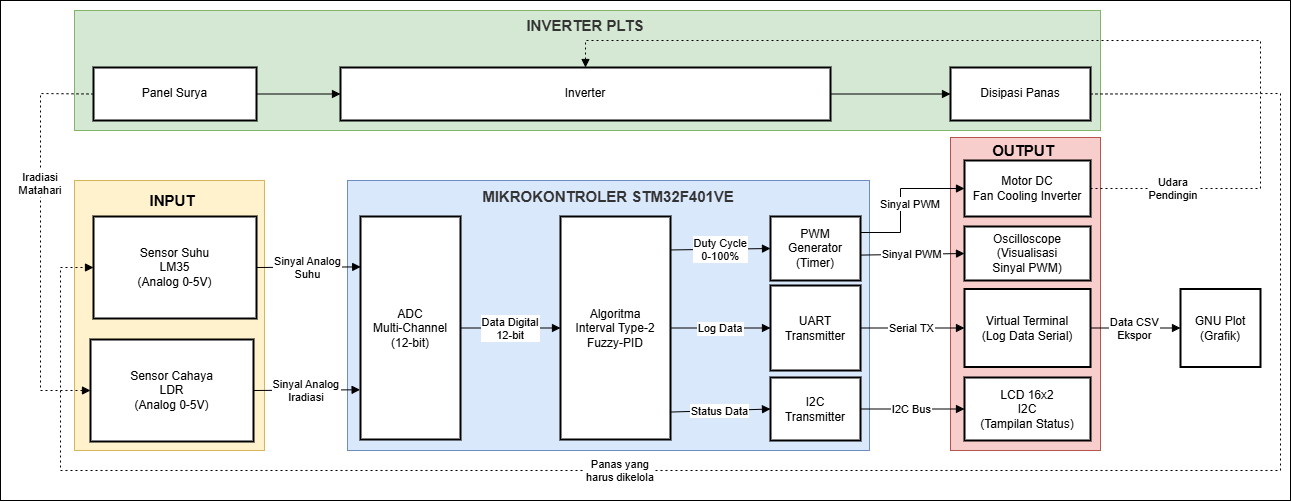
\includegraphics[width=\textwidth]{diagramblok.png}
\caption{Diagram Blok Arsitektur Simulasi Software-in-the-Loop Sistem Manajemen Termal Interval Type-2 Fuzzy-PID pada Inverter PLTS Berbasis STM32F401VE.}
\label{fig:diagram_blok}
\end{figure}

Diagram blok pada Figure 1 menggambarkan arsitektur keseluruhan sistem manajemen termal inverter PLTS yang disimulasikan dalam lingkungan \textit{Software-in-the-Loop} (SIL) menggunakan Proteus VSM. Sistem ini terdiri dari enam blok utama:

\begin{enumerate}
    \item \textbf{Blok Sensor (Input)} berisi dua sensor analog, yaitu sensor suhu LM35 yang membaca temperatur permukaan inverter dalam rentang 0--5V, dan sensor cahaya LDR yang membaca intensitas iradiasi matahari. Kedua sensor ini berfungsi sebagai masukan utama bagi sistem kendali.
    
    \item \textbf{Blok Mikrokontroler STM32F401VE} merupakan inti pemrosesan sistem. Di dalamnya terdapat modul ADC \textit{multi-channel} 12-bit yang mengonversi sinyal analog dari kedua sensor menjadi data digital, algoritma \textit{Interval Type-2 Fuzzy-PID} yang menghitung nilai \textit{duty cycle} optimal untuk kipas pendingin, modul \textit{PWM Generator} yang menghasilkan sinyal modulasi lebar pulsa, modul \textit{UART Transmitter} untuk pengiriman data serial ke \textit{Virtual Terminal}, serta modul \textit{I2C Transmitter} untuk komunikasi dengan LCD.
    
    \item \textbf{Blok Aktuator (Output)} berisi motor DC yang berfungsi sebagai kipas pendingin inverter. Kecepatan putaran motor diatur secara proporsional oleh sinyal PWM sesuai kebutuhan pendinginan.
    
    \item \textbf{Blok Display} berisi LCD 16x2 berbasis komunikasi I2C yang menampilkan informasi status sistem secara langsung, meliputi suhu aktual, nilai \textit{setpoint}, dan persentase \textit{duty cycle} kipas.
    
    \item \textbf{Blok Monitoring dan Instrumentasi} terdiri dari \textit{Virtual Terminal} yang menampilkan \textit{log} data serial secara \textit{real-time} dan \textit{Oscilloscope} yang memvisualisasikan bentuk gelombang sinyal PWM keluaran sistem.
    
    \item \textbf{Blok Analisis Data} menggunakan GNU Plot untuk menyajikan data simulasi dalam bentuk grafik respons, seperti grafik suhu, PWM, dan \textit{error} terhadap waktu. Data ini diperoleh dari ekspor \textit{log Virtual Terminal} dalam format CSV.
\end{enumerate}

Hubungan antara sistem pendingin dengan inverter PLTS ditunjukkan oleh garis putus-putus. Panel surya menghasilkan daya yang diproses oleh inverter, dan proses konversi daya ini menghasilkan disipasi panas. Panas tersebut dideteksi oleh sensor LM35, sementara intensitas iradiasi matahari dibaca oleh sensor LDR. Motor DC kipas pendingin kemudian mengarahkan aliran udara ke inverter untuk menurunkan suhu. Mekanisme \textit{closed-loop} inilah yang membentuk inti dari manajemen termal sistem.

\subsection*{2. Flowchart Algoritma}

% === Definisi Style ===
\tikzstyle{startstop} = [ellipse, minimum width=3cm, minimum height=1cm, text centered, draw=black, fill=red!15, font=\footnotesize\bfseries]
\tikzstyle{process} = [rectangle, minimum width=5cm, minimum height=0.8cm, text centered, draw=black, fill=blue!8, font=\footnotesize, text width=5.5cm]
\tikzstyle{io} = [trapezium, trapezium left angle=70, trapezium right angle=110, minimum width=4cm, minimum height=0.8cm, text centered, draw=black, fill=green!10, font=\footnotesize, text width=4.5cm]
\tikzstyle{decision} = [diamond, minimum width=2.5cm, minimum height=1cm, text centered, draw=black, fill=yellow!15, font=\footnotesize, aspect=2.5, text width=3cm]
\tikzstyle{connector} = [circle, minimum size=0.8cm, text centered, draw=black, fill=orange!20, font=\footnotesize\bfseries]
\tikzstyle{arrow} = [-{Stealth[length=2.5mm]}, thick]

% ============================================================
% HALAMAN 1: Flowchart Bagian Atas
% ============================================================
\begin{figure}[H]
\centering
\begin{tikzpicture}[node distance=1.1cm]

\node (start) [startstop] {START};

\node (init) [process, below=of start] {Inisialisasi Sistem\\Clock HSI 16 MHz, GPIO, ADC 12-bit,\\PWM 100 Hz, UART 4800 baud, I2C LCD};

\node (param) [process, below=of init] {Set Parameter Awal\\Setpoint Suhu = 50\textdegree C\\Referensi Cahaya = 500 Lux\\Gain PID: Kp=4.0, Ki=0.02, Kd=1.0};

\node (baca) [io, below=of param] {Baca Sensor Suhu (LM35)\\dan Sensor Cahaya (LDR)\\melalui ADC};

\node (fuzz) [process, below=of baca] {Fuzzifikasi \textit{Interval Type-2}\\Suhu \& Cahaya dipetakan ke\\3 himpunan (LOW, MED, HIGH)\\dengan \textit{Upper \& Lower} MF};

\node (rule) [process, below=of fuzz] {Evaluasi 9 Aturan Fuzzy\\Firing Strength = MIN($\mu_{suhu}$, $\mu_{cahaya}$)\\untuk Upper dan Lower};

\node (tr) [process, below=of rule] {\textit{Type Reduction} (Karnik-Mendel)\\dan Defuzzifikasi\\$\rightarrow$ menghasilkan \textit{Fuzzy Gain}};

\node (adapt) [process, below=of tr] {Hitung \textit{Adaptive Setpoint}\\adaptive\_sp = 50 + (500 $-$ cahaya) $\times$ 0.02};

\node (pid) [process, below=of adapt] {Komputasi PID\\error = suhu $-$ adaptive\_sp\\integral += error $\times$ 0.25\\U = fuzzy\_gain $\times$ (Kp$\cdot$e + Ki$\cdot\int$e + Kd$\cdot$de)};

\node (connA) [connector, below=of pid] {A};

% === ARROWS ===
\draw [arrow] (start) -- (init);
\draw [arrow] (init) -- (param);
\draw [arrow] (param) -- (baca);
\draw [arrow] (baca) -- (fuzz);
\draw [arrow] (fuzz) -- (rule);
\draw [arrow] (rule) -- (tr);
\draw [arrow] (tr) -- (adapt);
\draw [arrow] (adapt) -- (pid);
\draw [arrow] (pid) -- (connA);

\end{tikzpicture}
\end{figure}

\clearpage

% ============================================================
% HALAMAN 2: Flowchart Bagian Bawah
% ============================================================
\begin{figure}[H]
\centering
\begin{tikzpicture}[node distance=1.1cm]

\node (connA) [connector] {A};

\node (cek) [decision, below=1cm of connA] {Saturasi\\Nilai U?};

\node (max) [process, right=1.8cm of cek, text width=2.5cm, minimum width=2.8cm] {U = 999\\(Maksimum)};
\node (min) [process, left=1.8cm of cek, text width=2.5cm, minimum width=2.8cm] {U = 0\\(Minimum)};

\node (pwm) [io, below=1.5cm of cek] {Output PWM ke Motor DC\\(Atur Kecepatan \textit{Cooling Fan})};

\node (led) [decision, below=1.2cm of pwm] {PWM $>$ 350?};

\node (merah) [process, right=1.5cm of led, text width=2.5cm, minimum width=2.8cm] {LED Merah ON\\(Beban Berat)};
\node (hijau) [process, left=1.5cm of led, text width=2.5cm, minimum width=2.8cm] {LED Hijau ON\\(Normal)};

\node (uart) [io, below=1.5cm of led] {Kirim Data ke\\Virtual Terminal (UART)};

\node (lcd) [io, below=of uart] {Tampilkan Data di\\LCD I2C 16$\times$2};

\node (osc) [io, below=of lcd] {Visualisasi Sinyal PWM\\di \textit{Oscilloscope} Proteus};

\node (gnu) [io, below=of osc] {Ekspor Data CSV\\untuk Grafik GNU Plot};

\node (delay) [process, below=of gnu] {Tunggu Periode Sampling ($\Delta t$)};

\node (loop) [process, below=of delay, text width=4cm] {Loop - Kembali ke Pembacaan Sensor\\(Blok``Baca Sensor'')};

% === ARROWS ===
\draw [arrow] (connA) -- (cek);

\draw [arrow] (cek) -- node[anchor=south, font=\scriptsize] {Ya, U $>$ 999} (max);
\draw [arrow] (cek) -- node[anchor=south, font=\scriptsize] {Ya, U $<$ 0} (min);
\draw [arrow] (cek) -- node[anchor=east, font=\scriptsize] {0 $\leq$ U $\leq$ 999} (pwm);
\draw [arrow] (max) |- (pwm);
\draw [arrow] (min) |- (pwm);

\draw [arrow] (pwm) -- (led);
\draw [arrow] (led) -- node[anchor=south, font=\scriptsize] {Ya} (merah);
\draw [arrow] (led) -- node[anchor=south, font=\scriptsize] {Tidak} (hijau);
\draw [arrow] (merah) |- (uart);
\draw [arrow] (hijau) |- (uart);

\draw [arrow] (uart) -- (lcd);
\draw [arrow] (lcd) -- (osc);
\draw [arrow] (osc) -- (gnu);
\draw [arrow] (gnu) -- (delay);
\draw [arrow] (delay) -- (loop);

\node (end) [startstop, right=2.3cm of delay] {END};
\draw [arrow] (delay) -- node[anchor=south, font=\scriptsize] {Daya Dimatikan} (end);


\end{tikzpicture}
\caption{\textit{Flowchart} Algoritma \textit{Interval Type-2 Fuzzy-PID}}
\label{fig:flowchart2}
\end{figure}

\noindent \textit{Flowchart} pada Figure 2 menggambarkan alur kerja algoritma kendali \textit{Interval Type-2 Fuzzy-PID} yang dieksekusi secara berulang pada mikrokontroler STM32 virtual di dalam lingkungan simulasi Proteus.

\begin{enumerate}
    \item \textbf{Inisialisasi Sistem.} Ketika sistem dinyalakan, mikrokontroler mengonfigurasi seluruh periferal yang diperlukan, meliputi \textit{clock} prosesor HSI pada 16 MHz, modul ADC 12-bit untuk pembacaan sensor, \textit{timer} PWM pada frekuensi 100 Hz, komunikasi UART pada \textit{baud rate} 4800 untuk transmisi data serial, serta komunikasi I2C untuk layar LCD 16$\times$2.

    \item \textbf{Set Parameter Awal.} Sebelum memasuki siklus utama, sistem menetapkan parameter kendali yang terdiri dari \textit{setpoint} suhu sebesar 50\textdegree C sebagai target temperatur operasi inverter, nilai referensi cahaya sebesar 500 Lux sebagai titik tengah penyesuaian adaptif, serta \textit{gain} PID awal yaitu Kp = 4.0, Ki = 0.02, dan Kd = 1.0.

    \item \textbf{Pembacaan Sensor.} Pada setiap siklus, sistem membaca dua masukan analog melalui ADC. Sensor suhu LM35 mengukur temperatur permukaan inverter dan mengonversinya ke satuan derajat Celsius dengan rumus: $T = \frac{\text{raw} \times 100}{4095}$. Sensor cahaya LDR mengukur intensitas iradiasi matahari dan mengonversinya ke satuan Lux dengan rumus: $L = \frac{\text{raw} \times 1000}{4095}$.

    \item \textbf{Fuzzifikasi \textit{Interval Type-2}.} Kedua nilai sensor dipetakan ke dalam tiga himpunan fuzzy linguistik: LOW, MEDIUM, dan HIGH. Setiap himpunan memiliki dua fungsi keanggotaan, yaitu \textit{Upper Membership Function} dan \textit{Lower Membership Function}, yang bersama-sama membentuk \textit{Footprint of Uncertainty} (FOU). Struktur ganda ini memungkinkan sistem menangani ketidakpastian pembacaan sensor secara otomatis.

    \item \textbf{Evaluasi 9 Aturan Fuzzy.} Sembilan aturan IF-THEN yang merupakan kombinasi dari 3 himpunan suhu $\times$ 3 himpunan cahaya dievaluasi menggunakan operasi MIN untuk menentukan \textit{firing strength} masing-masing aturan, baik pada jalur \textit{upper} maupun \textit{lower}.

    \item \textbf{\textit{Type Reduction} dan Defuzzifikasi.} Proses \textit{type reduction} menggunakan metode Karnik-Mendel menghitung rata-rata tertimbang dari kedua jalur:
    \begin{equation}
        y_{upper} = \frac{\sum w_U \cdot g}{\sum w_U}, \quad y_{lower} = \frac{\sum w_L \cdot g}{\sum w_L}
    \end{equation}
    Nilai \textit{fuzzy gain} akhir diperoleh melalui defuzzifikasi: $\text{fuzzy\_gain} = \frac{y_{upper} + y_{lower}}{2}$.

    \item \textbf{Hitung \textit{Adaptive Setpoint}.} Nilai \textit{setpoint} suhu disesuaikan secara adaptif berdasarkan kondisi cahaya:
    \begin{equation}
        \text{adaptive\_sp} = 50 + (500 - \text{cahaya}) \times 0.02
    \end{equation}
    Ketika cahaya rendah (di bawah 500 Lux), \textit{setpoint} dinaikkan sehingga kipas bekerja lebih agresif. Sebaliknya, ketika cahaya tinggi, \textit{setpoint} diturunkan.

    \item \textbf{Komputasi PID.} Sinyal kendali $U$ dihitung berdasarkan persamaan PID yang diperkuat oleh \textit{fuzzy gain}:
    \begin{equation}
        \text{error} = \text{suhu} - \text{adaptive\_sp}
    \end{equation}
    \begin{equation}
        U = \text{fuzzy\_gain} \times (K_p \cdot e + K_i \cdot \textstyle\int e + K_d \cdot \Delta e)
    \end{equation}
    Mekanisme \textit{anti-windup} membatasi akumulasi integral pada rentang $\pm 300$ untuk mencegah lonjakan berlebihan.

    \item \textbf{Saturasi Output.} Nilai $U$ dibatasi pada rentang 0--999 untuk memastikan sinyal PWM tidak melebihi kapasitas aktuator. Apabila $U > 999$, nilai diatur ke 999 (maksimum). Apabila $U < 0$, nilai diatur ke 0 (minimum).

    \item \textbf{Output PWM dan Indikator LED.} Nilai $U$ dikonversi menjadi \textit{duty cycle} PWM yang mengatur kecepatan putaran motor DC kipas pendingin inverter. Indikator LED memberikan informasi visual: LED merah menyala apabila PWM $>$ 350 (beban berat) dan LED hijau menyala apabila PWM $\leq$ 350 (kondisi normal).

    \item \textbf{Monitoring dan Analisis Data.} Data operasi yang meliputi suhu, cahaya, PWM, dan tegangan motor disajikan melalui empat Channel:
    \begin{itemize}
        \item Data dikirim via UART ke \textit{Virtual Terminal} untuk pencatatan log serial.
        \item Informasi ditampilkan pada layar LCD I2C 16$\times$2 untuk pemantauan langsung.
        \item Sinyal PWM divisualisasikan pada \textit{Oscilloscope} Proteus untuk verifikasi bentuk gelombang.
        \item Data log diekspor dalam format CSV untuk dianalisis dalam bentuk grafik menggunakan GNU Plot.
    \end{itemize}

    \item \textbf{Periode Sampling dan \textit{Loop}.} Setelah seluruh proses selesai, sistem menunggu selama satu periode sampling ($\Delta t$) sebelum kembali ke tahap pembacaan sensor dan mengulangi seluruh siklus kendali secara terus-menerus. Siklus ini hanya berhenti apabila daya sistem dimatikan.
\end{enumerate}

\newpage
% ============================================================
% BAB C - SIMULASI DAN HASIL
% ============================================================

\newpage
\section*{C. Simulasi dan Hasil}

Bagian ini menjelaskan lingkungan simulasi, perangkat lunak yang digunakan,
rangkaian sistem virtual, serta hasil pengujian algoritma Interval Type-2
Fuzzy-PID pada sistem manajemen termal inverter PLTS berbasis STM32F401VE.
Seluruh pengujian dilakukan menggunakan pendekatan
\textit{Software-in-the-Loop} (SIL) pada Proteus VSM.

% ============================================================
\subsection*{1. Alat dan Perangkat Lunak}
Penelitian ini dilaksanakan sepenuhnya dalam lingkungan simulasi berbasis
perangkat lunak (\textit{Software-in-the-Loop}/SIL), sehingga tidak memerlukan
pengadaan komponen fisik. Seluruh proses perancangan, pemrograman, dan pengujian
sistem dilakukan menggunakan kombinasi perangkat lunak yang saling terintegrasi.
Berikut merupakan perangkat lunak dan platform yang digunakan dalam penelitian.
% ----------------------------------------------------------
\subsubsection*{1.1 Proteus 8 Professional}
\noindent\textbf{Fungsi dalam Sistem:}\\
Proteus 8 Professional digunakan sebagai platform simulasi elektronik utama
dalam penelitian ini. Seluruh rangkaian sistem manajemen termal inverter PLTS
dirancang dan dijalankan di dalam lingkungan Proteus VSM
(\textit{Virtual System Modelling}).
\vspace{6pt}

\noindent\textbf{Spesifikasi Teknis:}
\begin{itemize}
    \item Versi: Proteus 8 Professional
    \item Fitur utama:
    \begin{itemize}
        \item \textit{Virtual System Modelling} (VSM) untuk simulasi mikrokontroler
        \item \textit{Virtual Terminal} untuk monitoring data serial
        \item \textit{Virtual Oscilloscope} untuk visualisasi sinyal PWM
        \item Dukungan simulasi STM32 ARM Cortex-M4
    \end{itemize}
\end{itemize}
\vspace{6pt}
\noindent\textbf{Alasan Pemilihan:}\\
Proteus mendukung eksekusi langsung file \texttt{.hex} pada mikrokontroler
virtual STM32 sehingga sangat sesuai untuk pendekatan
\textit{Software-in-the-Loop}.
% ----------------------------------------------------------
\subsubsection*{1.2 Keil \textmu{}Vision}
\noindent\textbf{Fungsi dalam Sistem:}\\
Keil \textmu{}Vision digunakan sebagai IDE (\textit{Integrated Development Environment})
untuk menulis, mengompilasi, dan membangun kode \textit{firmware} sistem berbasis bahasa C.
\vspace{6pt}

\noindent\textbf{Spesifikasi Teknis:}
\begin{itemize}
    \item Platform target: ARM Cortex-M4
    \item Bahasa pemrograman: C
    \item Toolchain: ARM Compiler 6 (armclang)
    \item Output: File \texttt{.hex} untuk Proteus
\end{itemize}
\vspace{6pt}
\noindent\textbf{Alasan Pemilihan:}\\
Keil memiliki kompatibilitas tinggi dengan seri mikrokontroler STM32 dan mendukung
integrasi langsung dengan STM32CubeMX untuk konfigurasi periferal.
% ----------------------------------------------------------
\subsubsection*{1.3 STM32CubeMX}
\noindent\textbf{Fungsi dalam Sistem:}\\
STM32CubeMX digunakan untuk konfigurasi awal periferal STM32F401VE secara grafis
dan menghasilkan kode inisialisasi dasar sebagai kerangka proyek.
\vspace{6pt}

\noindent\textbf{Periferal yang Dikonfigurasi:}
\begin{itemize}
    \item ADC \textit{multi-channel} 12-bit (Chanel 0 dan Chanel 1)
    \item PWM Timer (TIM1 Channel 1)
    \item UART (USART2, 4800 baud)
    \item GPIO (LED indikator dan arah motor)
    \item Clock: HSI 16 MHz
\end{itemize}
\vspace{6pt}
\noindent\textbf{Alasan Pemilihan:}\\
STM32CubeMX mempermudah konfigurasi register STM32 secara visual dan mengurangi
kesalahan konfigurasi perangkat keras tingkat rendah.
% ----------------------------------------------------------
\subsubsection*{1.4 GNUPlot}
\noindent\textbf{Fungsi dalam Sistem:}\\
GNUPlot digunakan untuk visualisasi data hasil simulasi dalam bentuk grafik
ilmiah berbasis data CSV yang diekspor dari \textit{Virtual Terminal} Proteus.
\vspace{6pt}

\noindent\textbf{Data yang Dianalisis:}
\begin{itemize}
    \item Grafik suhu terhadap waktu
    \item Grafik \textit{duty cycle} PWM terhadap waktu
    \item Grafik \textit{error} kendali terhadap waktu
    \item Grafik respons sistem keseluruhan
\end{itemize}
\vspace{6pt}
\noindent\textbf{Alasan Pemilihan:}\\
GNUPlot mampu menghasilkan grafik ilmiah beresolusi tinggi dan mendukung analisis
data berbasis CSV secara otomatis.
% ----------------------------------------------------------
\subsubsection*{1.5 Mikrokontroler Virtual STM32F401VE}
\noindent\textbf{Fungsi dalam Sistem:}\\
STM32F401VE digunakan sebagai pusat pemrosesan utama sistem manajemen termal
dalam lingkungan simulasi Proteus.
\begin{table}[H]
    \centering
    \caption{Spesifikasi Teknis STM32F401VE}
    \label{tab:spesifikasi_stm32}
    \renewcommand{\arraystretch}{1.3}
    \begin{tabular}{>{\bfseries}p{6cm} p{7.5cm}}
        \toprule
        Parameter & Spesifikasi \\
        \midrule
        Seri & STM32F401VE \\
        Arsitektur & ARM Cortex-M4 dengan FPU \\
        Clock Maksimum & 84 MHz \\
        Clock yang Digunakan & HSI 16 MHz (tanpa PLL) \\
        Flash Memory & 512 KB \\
        RAM & 96 KB \\
        Resolusi ADC & 12-bit \\
        Frekuensi PWM & 100 Hz (Prescaler 159, Period 999) \\
        Komunikasi Serial & UART 4800 baud (USART2) \\
        Komunikasi Display & Soft I2C (PB8/SCL, PB9/SDA) \\
        \bottomrule
    \end{tabular}
\end{table}
\vspace{6pt}
\noindent\textbf{Alasan Pemilihan:}\\
STM32F401VE memiliki unit \textit{floating-point} (FPU) bawaan yang memadai
untuk menjalankan operasi aritmatika algoritma \textit{Interval Type-2 Fuzzy-PID}
secara efisien.
% ----------------------------------------------------------
\subsubsection*{1.6 Komponen Virtual Proteus}
\noindent Selain mikrokontroler, beberapa komponen virtual berikut digunakan dalam
rangkaian simulasi Proteus.
\begin{table}[H]
    \centering
    \caption{Daftar Komponen Virtual dalam Simulasi Proteus}
    \label{tab:komponen_virtual}
    \renewcommand{\arraystretch}{1.3}
    \begin{tabular}{>{\bfseries}p{4cm} p{3cm} p{5.5cm}}
        \toprule
        Komponen & Pin STM32 & Fungsi \\
        \midrule
        Sensor Suhu LM35 & PA0 (ADC Ch.0) & Mengukur temperatur inverter (0--100\textdegree C) \\
        Sensor Cahaya LDR & PA1 (ADC Ch.1) & Mengukur iradiasi matahari (0--1000 Lux) \\
        Motor Driver L298 & PA8 (PWM), PB1, PB2 & Mengatur kecepatan kipas pendingin \\
        Motor DC & Via L298 & Kipas pendingin inverter \\
        LCD 16$\times$2 + PCF8574 & PB8 (SCL), PB9 (SDA) & Menampilkan data suhu, cahaya, PWM \\
        LED Hijau & PC13 & Indikator kondisi normal \\
        LED Merah & PC15 & Indikator beban berat (PWM $>$ 350) \\
        Virtual Terminal & PA2 (TX), PA3 (RX) & Log data serial 4800 baud \\
        Virtual Oscilloscope & PA8 & Visualisasi sinyal PWM \\
        \bottomrule
    \end{tabular}
\end{table}

% ==================================================================
% 2. RANGKAIAN SIMULASI
% ==================================================================

\subsection*{2. Rangkaian Simulasi}

Rangkaian simulasi dirancang di dalam Proteus 8 Professional menggunakan pendekatan \textit{Software-in-the-Loop} (SIL). Seluruh komponen yang digunakan merupakan komponen virtual yang tersedia di pustaka Proteus, dengan mikrokontroler STM32F401VE menjalankan file \texttt{.hex} hasil kompilasi dari Keil \textmu{}Vision.

% ----------------------------------------------------------
\subsubsection*{2.1 Topologi Rangkaian Keseluruhan}

\begin{figure}[H]
    \centering
    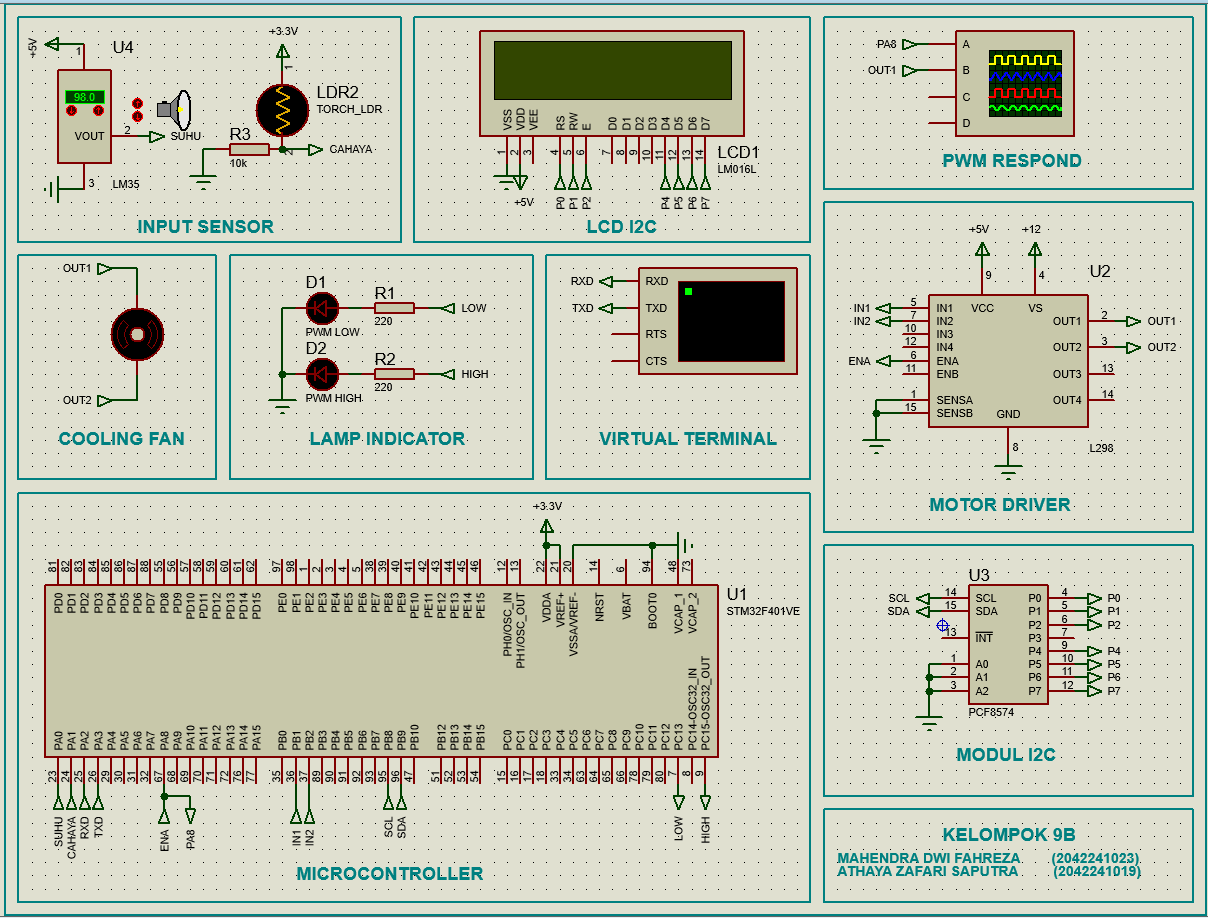
\includegraphics[width=\textwidth]{all.png}
    \caption{Rangkaian Keseluruhan Sistem di Proteus.}
    \label{fig:rangkaian_all}
\end{figure}

Gambar \ref{fig:rangkaian_all} menunjukkan topologi rangkaian lengkap yang terdiri dari beberapa blok fungsional. Masing-masing blok memiliki peran spesifik dalam rantai kendali \textit{Interval Type-2 Fuzzy-PID}, mulai dari akuisisi data sensor hingga aktuasi cooling fan dan pelaporan data.

% ----------------------------------------------------------
\subsubsection*{2.2 Blok Input Sensor}

\begin{figure}[H]
    \centering
    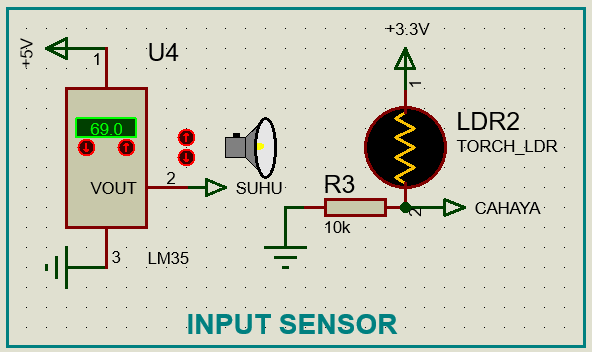
\includegraphics[width=7cm]{SENSOR.png}
    \caption{Blok Input Sensor.}
    \label{fig:sensor}
\end{figure}

Blok input terdiri dari dua sensor analog. Sensor suhu LM35 terhubung ke pin PA0 (ADC Channel 0) dengan pembagi tegangan resistor 1k$\Omega$ untuk penyesuaian skala. Sensor cahaya LDR terhubung ke pin PA1 (ADC Channel 1) dengan konfigurasi serupa. Kedua sinyal analog dikonversi oleh ADC 12-bit internal STM32 menjadi nilai digital pada rentang 0--4095. Firmware kemudian mengonversi nilai mentah tersebut menjadi satuan fisik melalui rumus:
\begin{equation}
    T_{\text{suhu}} = \frac{\text{raw\_adc} \times 100}{4095} \text{ (\textdegree C)}, \qquad
    L_{\text{cahaya}} = \frac{\text{raw\_adc} \times 1000}{4095} \text{ (Lux)}
\end{equation}

Kedua nilai ini menjadi masukan utama bagi tahap fuzzifikasi pada algoritma \textit{Interval Type-2 Fuzzy-PID}. Nilai suhu menentukan besarnya \textit{error} terhadap \textit{setpoint}, sedangkan nilai cahaya berfungsi sebagai variabel pengubah \textit{setpoint} secara adaptif.

% ----------------------------------------------------------
\subsubsection*{2.3 Blok Mikrokontroler}

\begin{figure}[H]
    \centering
    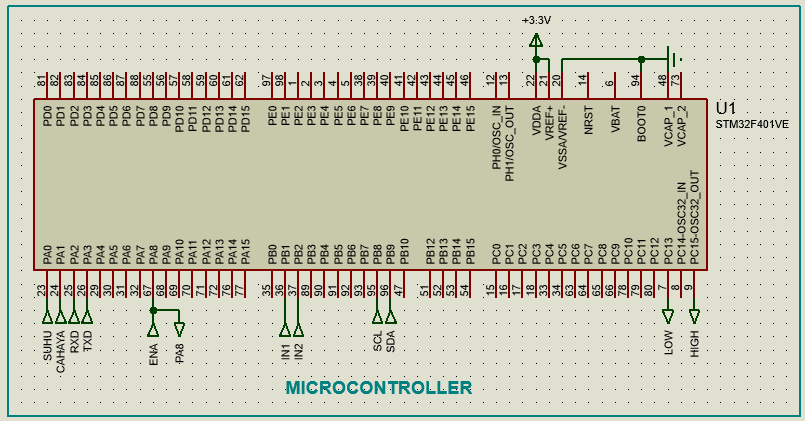
\includegraphics[width=17cm]{STM32.png}
    \caption{Blok mikrokontroler STM32F401VE dengan pemetaan pin periferal.}
    \label{fig:blok_mcu}
\end{figure}

Mikrokontroler STM32F401VE (U1) beroperasi pada \textit{clock} HSI 16 MHz tanpa PLL. Pin-pin yang digunakan dalam sistem dipetakan sebagai berikut:

\begin{table}[H]
    \centering
    \caption{Pemetaan pin STM32F401VE pada rangkaian simulasi.}
    \label{tab:pin_mapping}
    \renewcommand{\arraystretch}{1.2}
    \begin{tabular}{p{2cm} p{3cm} p{7cm}}
        \toprule
        \textbf{Pin} & \textbf{Fungsi} & \textbf{Keterangan} \\
        \midrule
        PA0 & ADC Channel 0 & Input sensor suhu LM35 \\
        PA1 & ADC Channel 1 & Input sensor cahaya LDR \\
        PA2 & USART2 TX & Transmisi data serial ke Virtual Terminal \\
        PA3 & USART2 RX & Penerimaan data serial \\
        PA8 & TIM1 CH1 PWM & Sinyal PWM ke Motor Driver L298 \\
        PB1 & GPIO Output & Arah putaran motor (IN1) \\
        PB2 & GPIO Output & Arah putaran motor (IN2) \\
        PB8 & Soft I2C SCL & \textit{Clock} komunikasi I2C ke PCF8574 \\
        PB9 & Soft I2C SDA & Data komunikasi I2C ke PCF8574 \\
        PC13 & GPIO Output & LED Hijau (indikator normal) \\
        PC15 & GPIO Output & LED Merah (indikator bahaya) \\
        \bottomrule
    \end{tabular}
\end{table}

Firmware yang tertanam mengimplementasikan arsitektur \textit{super-loop} dengan penjadwalan berbasis waktu menggunakan fungsi \texttt{HAL\_GetTick()}. Terdapat empat \textit{task} terjadwal: pembacaan sensor (1000 ms), perhitungan atau komputasi \textit{IT2 Fuzzy-PID} (500 ms), pembaruan atau \textit{update} perubahan aktuator dan perubahan LED (1000 ms), serta pengiriman data UART dan LCD (500 ms).

% ----------------------------------------------------------
\subsubsection*{2.4 Blok Aktuator (Motor Driver dan Kipas)}

\begin{figure}[H]
    \centering
    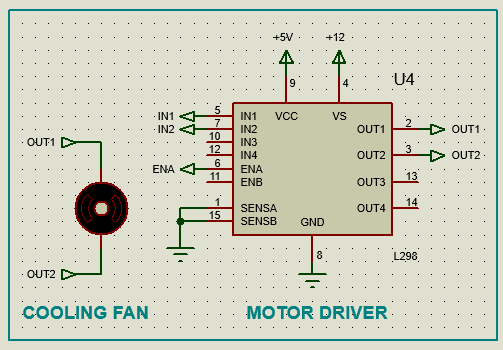
\includegraphics[width=9cm]{aktuator.png}
    \caption{Blok aktuator: IC L298 dan Motor DC sebagai \textit{Cooling Fan}.}
    \label{fig:blok_aktuator}
\end{figure}

IC Motor Driver L298 (U4) menerima sinyal PWM dari pin PA8 melalui pin ENA (\textit{Enable A}) untuk mengatur kecepatan putaran Motor DC. Pin IN1 dan IN2 (terhubung ke PB1 dan PB2) mengatur arah putaran motor, yang dalam konfigurasi ini ditetapkan satu arah saja. Motor DC disuplai oleh tegangan terpisah sebesar +12V melalui pin VS, sementara logika L298 disuplai +5V melalui pin VCC.

Nilai \textit{duty cycle} PWM yang dikirim ke ENA merupakan keluaran langsung dari algoritma \textit{Interval Type-2 Fuzzy-PID}, dengan rentang 0--999 yang merepresentasikan 0\%--100\% kecepatan putaran kipas. Estimasi tegangan motor dihitung oleh firmware sebagai:
\begin{equation}
    V_{\text{motor}} = \frac{\text{PWM} \times 12}{999} \text{ (Volt)}
\end{equation}

% ----------------------------------------------------------
\subsubsection*{2.5 Blok Display (LCD I2C dan Indikator LED)}

\begin{figure}[H]
    \centering
    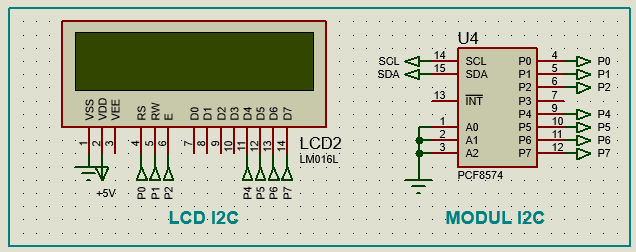
\includegraphics[width=10cm]{displaymonitoring.png}
    \caption{Blok display: LCD 16$\times$2 dengan modul I2C PCF8574.}
    \label{fig:blok_lcd}
\end{figure}

Modul LCD LM016L (16$\times$2 karakter) terhubung ke mikrokontroler melalui IC \textit{I/O Expander} PCF8574 yang berkomunikasi menggunakan protokol \textit{Soft I2C} pada pin PB8 (SCL) dan PB9 (SDA). Pada baris pertama LCD ditampilkan nilai suhu dan cahaya aktual, sedangkan baris kedua menampilkan nilai PWM dan estimasi tegangan motor.

Dua LED (pada blok Lamp Indicator) berfungsi sebagai indikator status beban:
\begin{itemize}
    \item \textbf{LED Hijau (PC13):} menyala ketika nilai PWM $\leq$ 350, menandakan operasi dalam kapasitas efisien.
    \item \textbf{LED Merah (PC15):} menyala ketika nilai PWM $>$ 350, menandakan beban pendinginan tinggi yang memerlukan perhatian.
\end{itemize}

% ----------------------------------------------------------
\subsubsection*{2.6 Blok Monitoring (Virtual Terminal dan Oscilloscope)}

\begin{figure}[H]
    \centering
    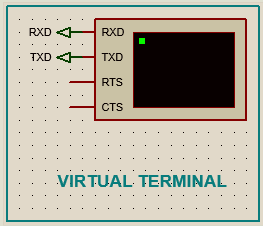
\includegraphics[width=5cm]{virtualmonitoring.png}
    \caption{Blok monitoring: Virtual Terminal untuk log data serial.}
    \label{fig:blok_terminal}
\end{figure}

Virtual Terminal Proteus terhubung ke pin PA2 (TX) dan PA3 (RX) dengan konfigurasi UART pada \textit{baud rate} 4800. Setiap 500 ms, firmware mengirimkan satu baris data log. Data ini dapat disalin dan diekspor ke format CSV untuk analisis lebih lanjut menggunakan GNUPlot.

\textit{Digital Oscilloscope} Proteus dihubungkan ke pin PA8 untuk memvisualisasikan bentuk gelombang PWM secara langsung. Channel A dan Channel B pada osiloskop menampilkan sinyal PWM dari sudut pandang yang berbeda, memungkinkan verifikasi frekuensi (100 Hz) dan variasi \textit{duty cycle} sesuai keluaran algoritma kendali.

% ==================================================================
% 3. HASIL PENGUJIAN SIMULASI
% ==================================================================

\subsection*{3. Hasil Pengujian Simulasi}

Pengujian dilakukan dengan mengubah nilai pembacaan sensor secara interaktif pada saat simulasi berjalan. Tiga skenario diuji untuk memverifikasi respons algoritma kendali pada kondisi yang berbeda.

% ----------------------------------------------------------
\subsubsection*{3.1 Respons Sistem pada Kondisi Beban Menengah}

\begin{figure}[H]
    \centering
    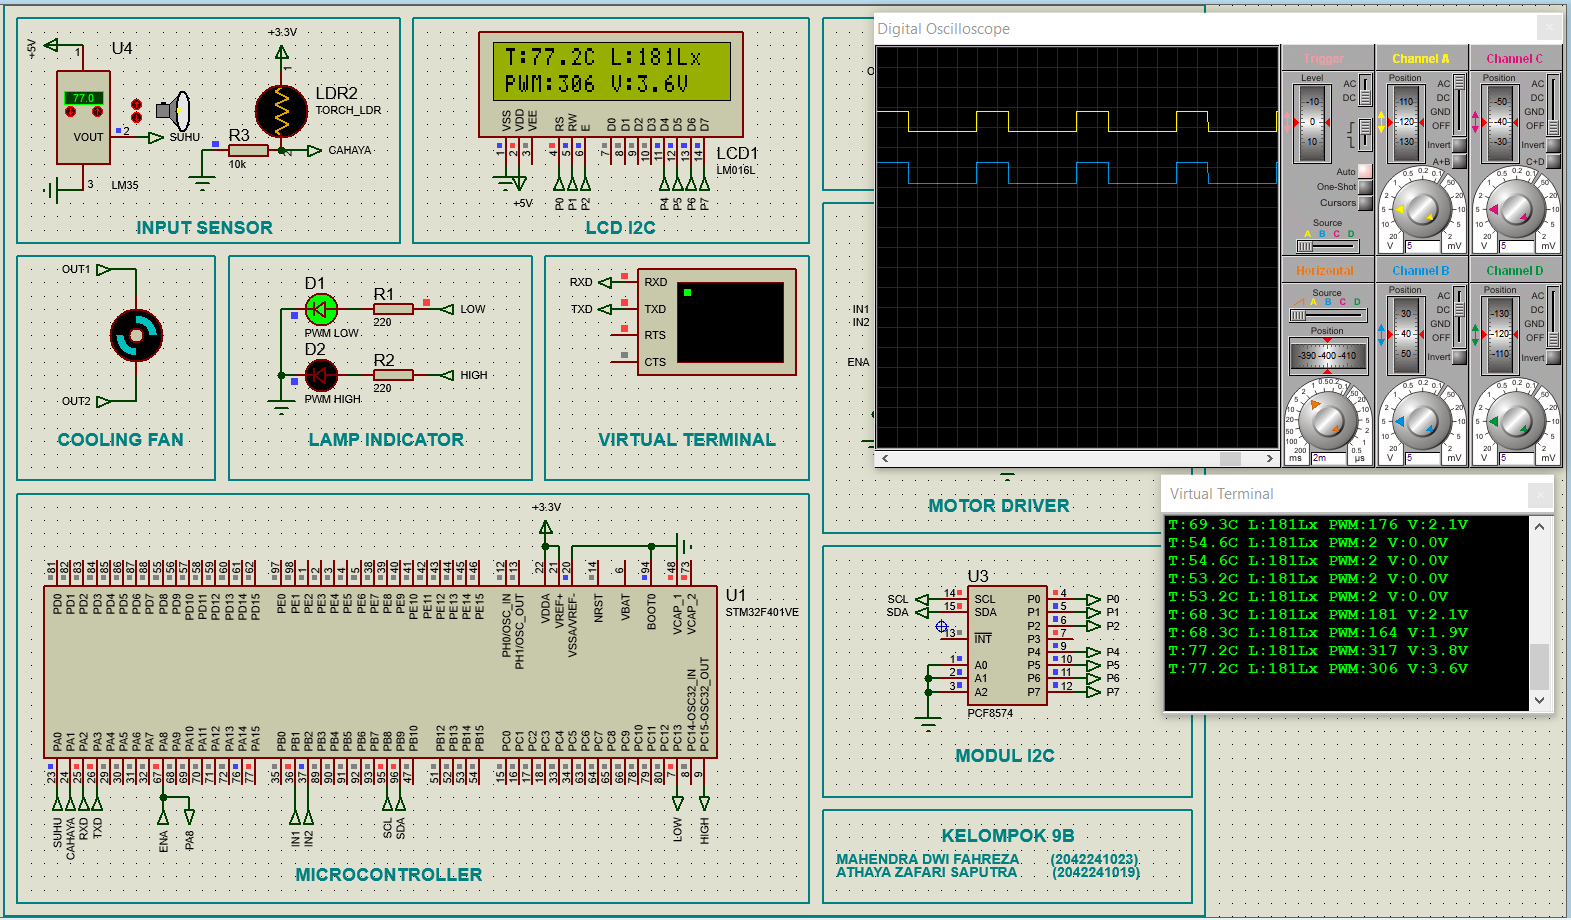
\includegraphics[width=16cm]{runtampilanall_normal.png}
    \caption{Tampilan keseluruhan simulasi pada kondisi operasi aman ($T = 77{,}2^\circ\text{C}$).}
    \label{fig:run_normal}
\end{figure}

\begin{figure}[H]
    \centering
    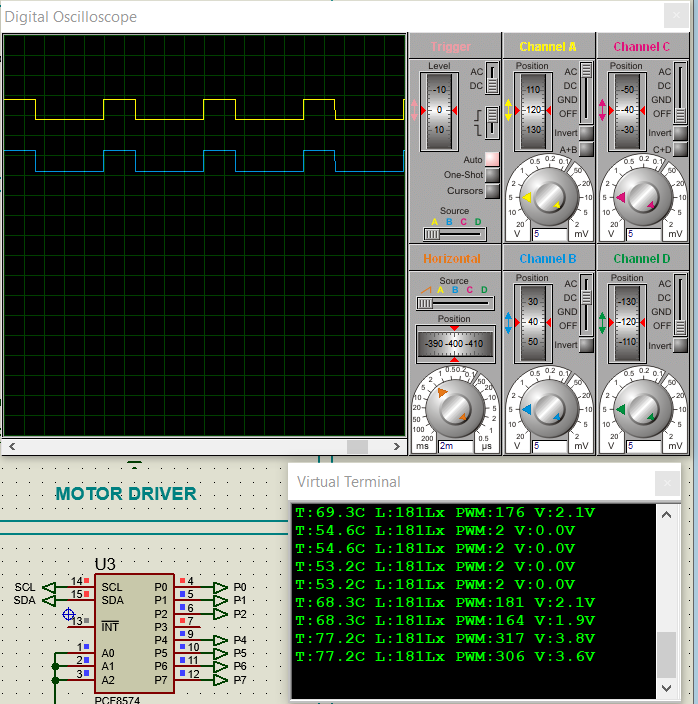
\includegraphics[width=12cm]{vmnormal.png}
    \caption{Virtual Terminal dan Oscilloscope pada kondisi operasi aman.}
    \label{fig:vm_normal}
\end{figure}

Pada pengujian pertama, sensor suhu LM35 menunjukkan pembacaan $T = 77{,}2^\circ\text{C}$ dan sensor cahaya LDR menunjukkan $L = 181\text{ Lux}$ (kondisi redup/mendung). Berdasarkan logika \textit{adaptive setpoint}, nilai \textit{setpoint} target suhu dihitung sebagai:
\begin{equation}
    \text{adaptive\_sp} = 50 + (500 - 181) \times 0{,}02 = 56{,}38^\circ\text{C}
\end{equation}

Suhu aktual ($77{,}2^\circ\text{C}$) telah melewati \textit{setpoint} adaptif ($56{,}38^\circ\text{C}$), menghasilkan \textit{error} positif sebesar $20{,}82^\circ\text{C}$. Namun, karena intensitas cahaya sangat rendah, \textit{Fuzzy Logic} menyimpulkan bahwa tidak ada radiasi panas eksternal, sehingga keluaran kendali dijaga pada tingkat moderat. Nilai PWM tercatat pada angka 306 dengan estimasi tegangan motor sebesar $V = 3{,}6\text{V}$. Karena parameter PWM $\leq 350$, sistem tetap mempertahankan indikator LED Hijau (Status Aman). Pada \textit{Virtual Oscilloscope}, bentuk gelombang memperlihatkan \textit{duty cycle} sebesar $30{,}6\%$, yang berarti kipas pendingin berputar pada kecepatan sedang untuk menjaga sirkulasi secara efisien.

% ----------------------------------------------------------
\subsubsection*{3.2 Respons Sistem pada Kondisi Beban Kritis}

\begin{figure}[H]
    \centering
    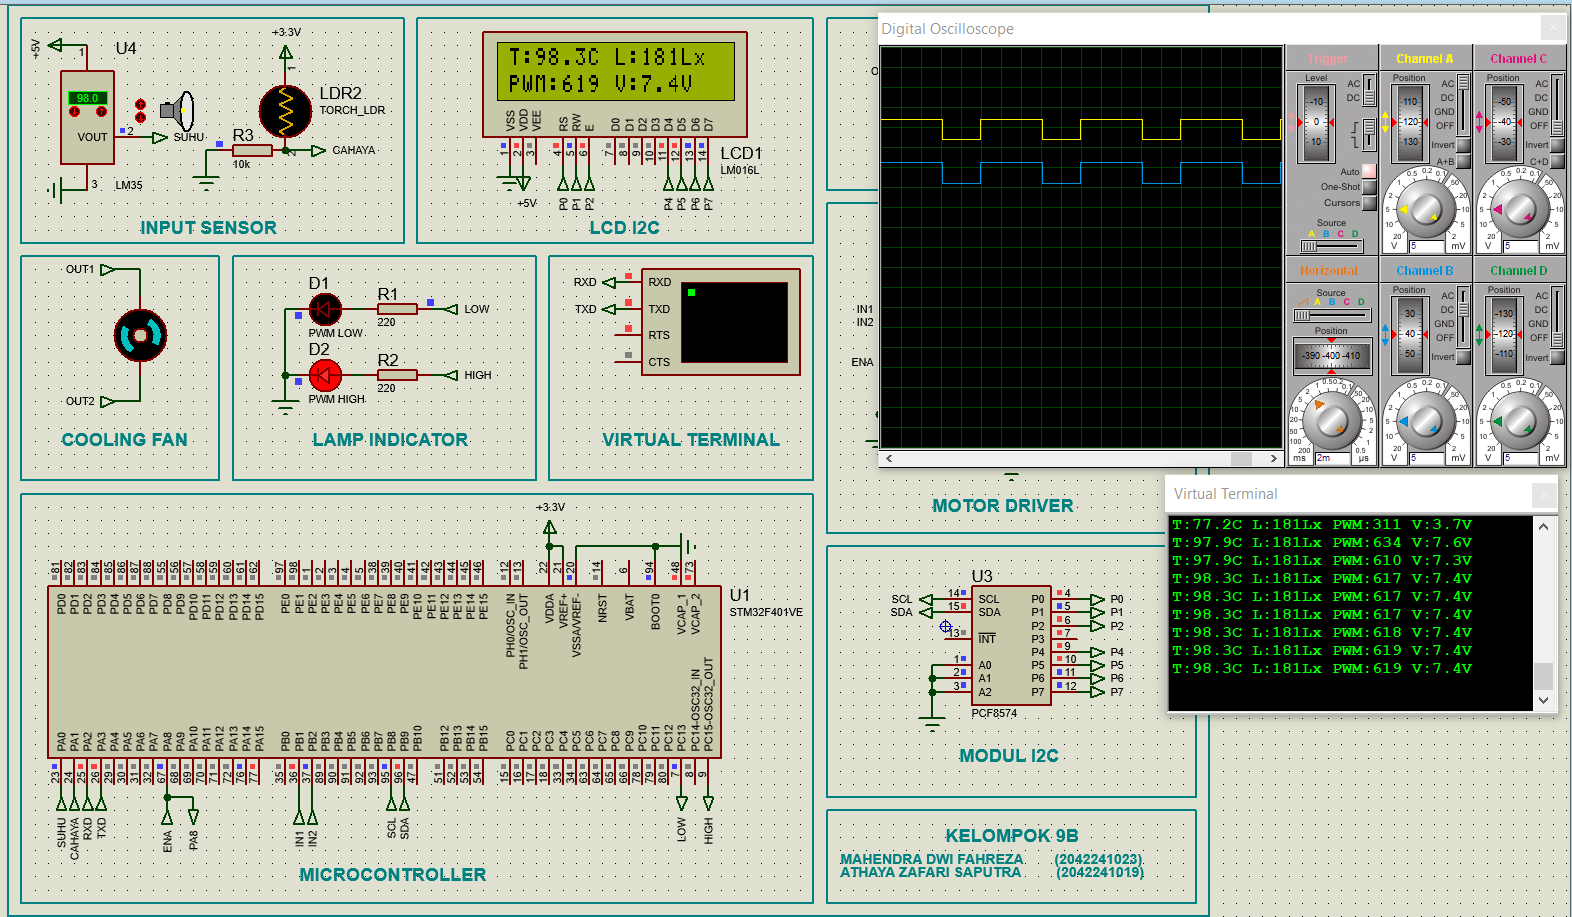
\includegraphics[width=16cm]{runtampilanall_bahaya.png}
    \caption{Tampilan keseluruhan simulasi pada kondisi suhu kritis ($T = 98{,}3^\circ\text{C}$).}
    \label{fig:run_bahaya}
\end{figure}

\begin{figure}[H]
    \centering
    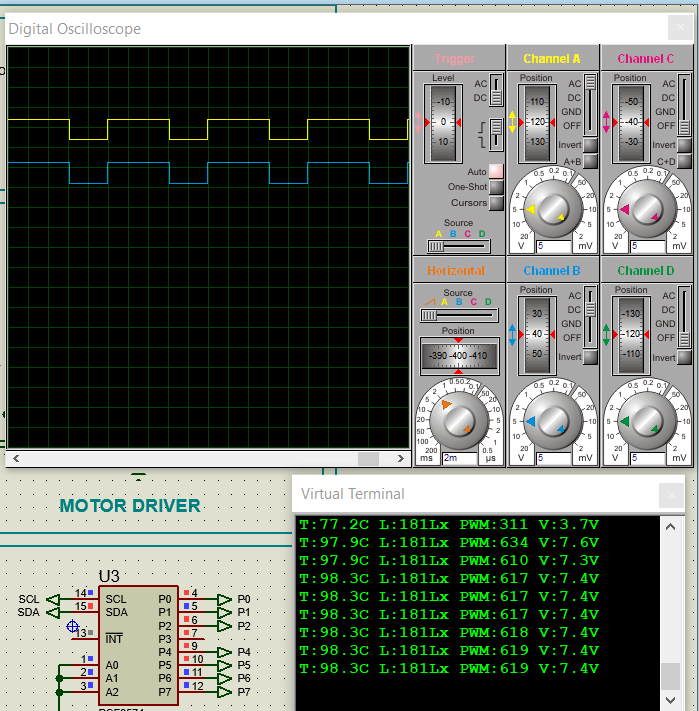
\includegraphics[width=12cm]{vmbahaya.png}
    \caption{Virtual Terminal dan Oscilloscope pada kondisi suhu kritis.}
    \label{fig:vm_bahaya}
\end{figure}

Pada pengujian kedua, kondisi beban puncak didemonstrasikan dengan mensimulasikan kenaikan suhu drastis hingga menyentuh batas kritis $T = 98{,}3^\circ\text{C}$, dengan intensitas cahaya tetap di $L = 181\text{ Lux}$. Pada kondisi ini, nilai \textit{setpoint} adaptif tetap bertahan di angka $56{,}38^\circ\text{C}$.

Hal ini menyebabkan \textit{error} kendali bernilai sangat besar dan positif ($98{,}3 - 56{,}38 = 41{,}92^\circ\text{C}$). Sebagai respons, keluaran PID yang diperkuat oleh komputasi \textit{Fuzzy Gain} memberikan hentakan daya keluaran yang signifikan untuk membuang panas. Nilai PWM tercatat melonjak tinggi ke angka 619, dengan estimasi tegangan suplai motor mencapai $V = 7{,}4\text{V}$. Indikator peringatan berubah seketika menjadi LED Merah yang menyala secara konsisten karena batas aman (PWM $> 350$) telah terlampaui. Pada \textit{Virtual Oscilloscope}, pelebaran gelombang pulsa PWM (\textit{Duty Cycle}) terlihat sangat jelas hingga mencapai $61{,}9\%$. Keluaran ekstrem ini memaksa kipas berputar kencang guna segera mendisipasi panas berlebih dari \textit{heatsink} dan mencegah kerusakan fisik pada komponen inverter.



\subsection*{4. Data dan Plot GNUPlot}
% ----------------------------------------------------------
\subsubsection*{4.1 Proses Ekstraksi dan Pengolahan Data}
Data hasil simulasi tidak diperoleh secara otomatis dalam bentuk grafik, melainkan diekstraksi melalui serangkaian tahapan pengolahan data. Proses ini melibatkan empat langkah utama:
\begin{enumerate}
    \item \textbf{Pengambilan Log Data (Virtual Terminal):} Saat simulasi berjalan di Proteus, mikrokontroler STM32 secara kontinu mengirimkan data berformat \textit{string} (contoh: \texttt{T:74.9C L:749Lx PWM:971 V:11.6V}) setiap interval 500 ms melalui antarmuka UART menuju komponen \textit{Virtual Terminal}.
    \item \textbf{Eksport Teks (TXT):} Seluruh log teks yang tercetak di layar \textit{Virtual Terminal} hasil simulasi disalin (di-\textit{copy}), kemudian disimpan ke dalam format teks mentah (\texttt{.txt}).
    \item \textbf{Konversi Format (CSV):} Data teks mentah tersebut dibersihkan dari karakter alfabet sehingga hanya menyisakan deret nilai numerik murni. Data ini disusun secara terstruktur ke dalam format matriks \textit{Comma-Separated Values} (\texttt{.csv}) yang terdiri dari kolom Waktu, Suhu, Cahaya, PWM, dan Tegangan.
    \item \textbf{Visualisasi Grafik (GNUPlot):} File CSV kemudian diumpankan ke dalam perangkat lunak \textbf{GNUPlot}. Dengan menggunakan serangkaian skrip perintah (file \texttt{.gp}), GNUPlot memproses matriks angka tersebut menjadi grafik matematis 2D dan 3D beresolusi tinggi guna keperluan analisis performa sistem kendali.
\end{enumerate}
Total data yang diekstraksi berjumlah 98 sampel waktu riil yang mencakup dinamika sistem mulai dari kondisi awal, beban puncak, hingga respons pengereman (transisi).
% ----------------------------------------------------------
% ----------------------------------------------------------
\subsubsection*{4.2 Analisis Dinamika Sistem Berdasarkan Waktu (2D Plot)}

\begin{figure}[H]
    \centering
    
\includegraphics[width=16.5cm]{plot_gabungan.png}
    \caption{Multiplot dinamika waktu: Suhu aktual, Intensitas Cahaya, Respons PWM, dan Tegangan Motor.}
    \label{fig:plot_gabungan}
\end{figure}

Grafik \textit{time-series} pada Gambar \ref{fig:plot_gabungan} mendemonstrasikan perilaku transien sistem kendali terhadap gangguan lingkungan. Terdapat tiga fase operasi yang diamati:
\begin{itemize}
    \item \textbf{Fase Normal ($t = 0-14$ detik):} Pada suhu ruangan $29{,}0^\circ\text{C}$, sistem mempertahankan status istirahat (PWM 105). Saat suhu dinaikkan secara artifisial ke $49{,}9^\circ\text{C}$ pada detik ke-7,5, PWM merespons moderat di angka 500, membuktikan bahwa sistem tidak bereaksi berlebihan jika suhu belum menembus \textit{setpoint} dinamis.
    \item \textbf{Fase Kritis ($t = 15-23$ detik \& $t = 35-45$ detik):} Ketika suhu dipaksa menyentuh zona kritis ($>70^\circ\text{C}$), terlihat lonjakan tajam eksponensial pada sinyal PWM hingga mencapai tingkat saturasi (914-999). 
    \item \textbf{Fase Pengereman ($t = 23,5$ detik \& $t = 45,5$ detik):} Penurunan suhu mendadak dari $71{,}9^\circ\text{C}$ kembali ke $30{,}9^\circ\text{C}$ memicu aksi \textit{derivative} yang agresif. Sinyal kendali (PWM) jatuh seketika ke angka 2 sebelum perlahan stabil di nilai 56, berfungsi sebagai rem termal guna mencegah efek \textit{overshoot} yang dapat memboroskan daya.
\end{itemize}

Selain ketiga variabel di atas, panel keempat pada Gambar \ref{fig:plot_gabungan} memvisualisasikan estimasi profil Tegangan Motor (Volt). Bentuk kurva tegangan yang ekuivalen sempurna dengan kurva PWM membuktikan bahwa perangkat lunak berhasil menerjemahkan komputasi kendali \textit{Interval Type-2 Fuzzy-PID} (rentang 0-999) secara proporsional linier menjadi aktuasi fisik, yaitu injeksi tegangan ke Motor DC kipas pendingin (rentang 0-12V).

% ----------------------------------------------------------
\subsubsection*{4.3 Korelasi \textit{Fuzzy Logic} dan \textit{Adaptive Setpoint} (Scatter Plot)}

\begin{figure}[H]
    \centering
    
\includegraphics[width=12.3cm]{plot_scatter_suhu.png}
    \caption{Korelasi Suhu terhadap PWM.}
    \label{fig:scatter_suhu}
\end{figure}

\begin{figure}[H]
    \centering
    
\includegraphics[width=12.3cm]{plot_scatter_cahaya.png}
    \caption{Korelasi Cahaya terhadap PWM.}
    \label{fig:scatter_cahaya}
\end{figure}

Gambar \ref{fig:scatter_suhu} memperlihatkan pola klasterisasi kendali (\textit{gain scheduling}). Titik-titik data terbagi rapi pada tiga zona: rendah (PWM $<200$), menengah (PWM $\approx 500$), dan tersaturasi penuh (PWM $>900$). Relasi linier-eksponensial ini memvalidasi kehalusan inferensi logika \textit{fuzzy} dibandingkan dengan saklar \textit{On/Off} konvensional.

Di sisi lain, fungsi sensor cahaya sebagai pengubah ambang batas (\textit{adaptive setpoint}) tervalidasi pada Gambar \ref{fig:scatter_cahaya}. Pada intensitas cahaya ekstrem (iradiasi $>700\text{ Lux}$), titik PWM cenderung dipaksa menumpuk di atas. Sebaliknya, pada kondisi redup, margin toleransi suhu dilonggarkan sehingga titik PWM terkonsentrasi di nilai yang sangat kecil guna menghemat konsumsi energi baterai PLTS.

% ----------------------------------------------------------
\subsubsection*{4.4 Permukaan Kendali 3D (\textit{3D Control Surface})}

\begin{figure}[H]
    \centering
    
\includegraphics[width=0.85\textwidth]{plot_surface_3d.png}
    \caption{Representasi 3D \textit{Control Surface} dari algoritma IT2 Fuzzy-PID.}
    \label{fig:plot_3d}
\end{figure}

Gambar \ref{fig:plot_3d} menyajikan grafik \textit{3D Control Surface} yang dirender menggunakan GNUPlot dengan interpolasi data riil menggunakan metode \textit{dgrid3d}. Sumbu-X mewakili perubahan suhu seketika (\textit{error}), sumbu-Y mewakili variabel gangguan cahaya (\textit{adaptive setpoint}), dan sumbu-Z merupakan respons final PWM ke aktuator.

Topografi melengkung pada bidang permukaan warna hijau ke kuning membuktikan adanya transisi aksi kendali yang kontinu secara proporsional. Namun, terdapat patahan curam (\textit{steep gradient}) menuju area berwarna merah di mana kombinasi suhu tinggi dan cahaya terik secara instan mendorong aktuator ke kapasitas putaran puncaknya. Bentuk topografi non-linier yang mulus dan bebas dari osilasi tajam ini merupakan karakteristik utama sekaligus keunggulan matematis dari himpunan \textit{Interval Type-2 Fuzzy} (IT2-FLS) dalam menangani ketidakpastian (\textit{uncertainties}) parameter operasional inverter termal.

\newpage
\section*{D. Keunggulan Metode}

Penelitian ini telah berhasil merancang dan menyimulasikan Sistem Manajemen Termal Inverter PLTS menggunakan algoritma \textit{Interval Type-2 Fuzzy-PID} (IT2 Fuzzy-PID) melalui pendekatan \textit{Software-in-the-Loop} (SIL) pada mikrokontroler STM32F401VE. Berdasarkan hasil pengujian dinamika waktu dan grafik \textit{3D control surface}, sistem terbukti mampu memberikan respons kendali yang sangat mulus (\textit{smooth transition}) dan bebas dari osilasi tajam. Algoritma ini secara dinamis mengkalibrasi kecepatan kipas pendingin dari kondisi istirahat hingga kapasitas puncak (PWM tersaturasi di atas 900) saat mendeteksi suhu kritis, serta melakukan pengereman aktuator secara instan saat terjadi penurunan suhu mendadak guna mencegah \textit{overshoot} pendinginan.

Jika dibandingkan dengan metode pada jurnal artikel acuan yang umumnya berfokus pada simulasi PC atau pengontrol berbasis \textit{embedded OS}, implementasi \textit{bare-metal} C/C++ pada arsitektur ARM Cortex-M4 dalam penelitian ini menawarkan beberapa keunggulan. Dari segi kecepatan eksekusi dan penggunaan memori, penjadwalan \textit{scheduling} \textit{super-loop} memastikan komputasi matematika \textit{Interval Type-2 Fuzzy Logic System} yang kompleks dapat dieksekusi dengan \textit{overhead} memori yang sangat minimal dan waktu respons deterministik. Dari kemudahan integrasi, penggunaan periferal standar industri (ADC, perangkat keras \textit{hardware} PWM \textit{Pulse Width Modulation}, dan I2C) membuatnya mudah diadopsi ke modul inverter komersial. Selanjutnya, dari aspek \textit{safety} (keamanan), sistem ini dilengkapi dengan proteksi \textit{thermal runaway} reaktif dan indikator visual LED yang beralih seketika mengikuti zona keamanan operasi, sehingga meminimalisir risiko kegagalan perangkat keras akibat beban berlebih.

Kontribusi orisinalitas utama dari penelitian ini terletak pada penggabungan inovatif dari konsep-konsep yang sebelumnya hanya menjadi rekomendasi \textit{future work} (penelitian lanjutan) pada berbagai literatur sebelumnya. Penelitian ini tidak hanya mengimplementasikan \textit{Interval Type-2 Fuzzy} untuk menangani ketidakpastian termal non-linier, tetapi secara pionir memadukannya dengan mekanisme \textit{Adaptive Setpoint} prediktif yang digerakkan oleh intensitas cahaya (iradiasi matahari eksternal). Pada sistem konvensional, pendinginan bersifat murni reaktif terhadap suhu absolut. Namun pada sistem yang diajukan ini, intensitas cahaya matahari digunakan untuk memprediksi potensi beban daya PLTS, sehingga sistem dapat memperketat atau melonggarkan toleransi suhu secara proaktif sebelum panas berlebih benar-benar terakumulasi. Penggabungan pendekatan prediktif-adaptif dan ketahanan \textit{Type-2 Fuzzy} ini merupakan kebaruan yang secara nyata meningkatkan efisiensi energi dan durabilitas termal inverter PLTS.

\newpage
\section*{E. Dokumentasi GitHub \& LinkedIn}
\noindent\textbf{Tautan Repositori GitHub:} \url{https://github.com/S00eb/fuzzytype2-pid-thermal} \\
\textbf{Unggahan LinkedIn:} \href{https://www.linkedin.com/posts/mahendradf_softwareintheloop-embeddedsystems-stm32-ugcPost-7463782181484724225-sNw3/}{LinkedIn Project Publication} \\

\begin{figure}[H]
    \centering
    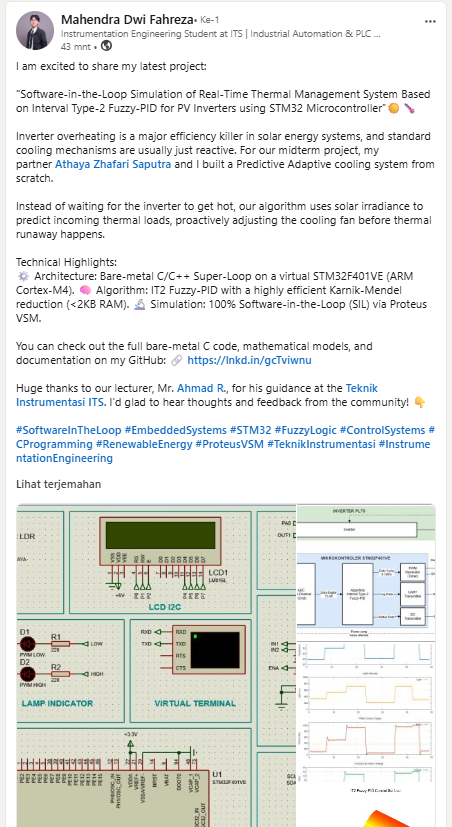
\includegraphics[width=0.50\textwidth]{publication_doc.png}
    \caption{Dokumentasi publikasi di Linkedin.}
    \label{fig:plot_3d}
\end{figure}

\newpage
\section*{F. Kesimpulan}
Tinjauan literatur terbaru menunjukan bahwa tren saat ini dalam pengembangan sistem kendali termal verfokus pada penggunaan algoritma cerdas yang adaptif pada mikrokontroler dengan memori terbatas dan kemampuan sistem untuk menagantisipasi secara proaktif ketidakpastian cuaca. Menjawab tantangan dari berbagai rekomendasi \textit{future work} tersebut, penelitian ini telah berhasil mengembangkan dan menyimulasikan sistem manajemen termal inverter PLTS menggunakan algoritma \textit{Interval Type-2 Fuzzy-PID} (IT2 Fuzzy-PID) pada mikrokontroler STM32F401VE. Inovasi kebaruan utama dari metode ini terletak pada penerapan \textit{Adaptive Setpoint} prediktif yang memanfaatkan pembacaan intensitas cahaya matahari eksternal guna mengantisipasi akumulasi panas berlebih sebelum terjadi secara reaktif.

Hasil pengujian \textit{Software-in-the-Loop} (SIL) membuktikan bahwa algoritma yang diajukan mampu memberikan respons kendali yang sangat mulus (\textit{smooth transition}) dan terhindar dari osilasi tajam. Sistem secara dinamis mengkalibrasi siklus kerja (\textit{duty cycle}) PWM dari kipas pendingin hingga mencapai batas saturasi maksimum di atas 900 saat beban termal memuncak. Di samping itu, sistem juga mampu mengerem aktuator secara instan pada saat terjadi penurunan suhu yang drastis, sehingga kejadian \textit{overshoot} pendinginan yang membuang energi secara sia-sia dapat dicegah. Keberhasilan ini menegaskan bahwa penggunaan struktur \textit{Footprint of Uncertainty} (FOU) sangat efektif dalam memodelkan ketidakpastian parameter lingkungan yang non-linier.

Secara arsitektural, implementasi \textit{bare-metal} C/C++ menggunakan pendekatan \textit{super-loop} terbukti sangat andal dalam menjalankan komputasi matematis kompleks \textit{Type-2 Fuzzy} dengan penggunaan \textit{overhead} memori yang sangat minimal pada prosesor ARM Cortex-M4. Mempertimbangkan tingginya stabilitas dan ketahanan yang ditunjukkan selama pengujian simulasi, pengembangan selanjutnya memiliki potensi yang sangat besar untuk diwujudkan dalam pengujian perangkat keras fisik (\textit{hardware-in-the-loop}). Selain itu, pengintegrasian sistem ini dengan jaringan telemetri berbasis \textit{Internet of Things} (IoT) sangat direkomendasikan guna mendukung fungsi pemantauan jarak jauh dan pelaporan status keandalan termal inverter secara \textit{real-time}.


\end{document}
